% concatenated from T13.tex
\documentclass[11pt]{article}

\usepackage[a4paper,margin=2.5cm]{geometry}
\usepackage[T1]{fontenc}
\usepackage{amsmath,amssymb,amsthm}
\usepackage{microtype}
\usepackage{tikz}
\usetikzlibrary{arrows.meta,calc,decorations.pathreplacing}
\usepackage[hidelinks]{hyperref}

\newcommand{\R}{\mathbb R}
\newcommand{\abs}[1]{\lvert #1\rvert}
\newcommand{\norm}[1]{\lVert #1\rVert}
\newcommand{\dist}{\operatorname{dist}}
\newcommand{\diam}{\operatorname{diam}}
\newcommand{\Tr}{\operatorname{Tr}}
\newcommand{\sgn}{\operatorname{sgn}}

\newtheorem{theorem}{Theorem}[section]
\newtheorem{lemma}[theorem]{Lemma}
\newtheorem{proposition}[theorem]{Proposition}
\newtheorem{corollary}[theorem]{Corollary}
\theoremstyle{definition}
\newtheorem{definition}[theorem]{Definition}
\theoremstyle{remark}
\newtheorem{remark}[theorem]{Remark}

\title{Rate of convergence of the $p$-torsion function to the distance function}

\author{Farid Bozorgnia\thanks{Department of Mathematics, New Uzbekistan University, Tashkent, Uzbekistan. Email: \texttt{f.bozorgnia@newuu.uz}}
\and
Masoud Bayrami-Aminlouee\thanks{Department of Mathematical Sciences, Sharif University of Technology, P.O.\ Box 11365-9415, Tehran, Iran; \texttt{masoud.bayrami1990@sharif.edu}. School of Mathematics, Institute for Research in Fundamental Sciences (IPM), P.O.\ Box 19395-5746, Tehran, Iran; \texttt{aminlouee@ipm.ir}}
\and
Khudoyor Mamayusupov\thanks{Department of Mathematics, New Uzbekistan University, Tashkent, Uzbekistan. Email: \texttt{k.mamayusupov@newuu.uz}}
}
\date{}

\begin{document}
\maketitle

\begin{abstract}
We prove that the Dirichlet $p$-torsion function $u_p$ converges to the
distance to the boundary $d$ at the rate $O(1/p)$ in the uniform norm, on
every bounded domain and with a constant depending only on the dimension and
the diameter. The upper bound comes from a radial barrier with its pole at a
boundary point, which is an admissible comparison function for $p>n$ and
needs no boundary regularity; the lower bound comes from an inscribed ball.
On the ball the error equals $(1+\log n)/p+O(p^{-2})$, so the order $1/p$
cannot be improved in general. Under a uniform exterior ball condition, an
annular barrier gives $u_p\le K_\Omega^{1/(p-1)}d$ for every $p>1$, with
$K_\Omega$ explicit in the dimension, the diameter and the exterior radius; on
convex sets the constant is the diameter, and a multiple of $d$ is a
supersolution whenever $-\Delta d$ has a positive distributional lower bound.
On $C^2$ domains, the same barrier and the classical gradient maximum principle
give $\norm{\nabla u_p}_{L^\infty}^{p-1}\le K_\Omega$. When $-\Delta d$ is a
measure of finite total variation, which we prove for $C^1$ domains with a
uniform exterior ball, the gradients converge in $L^q$ at the rate
$O(p^{-1/2})$ for $q\le2$ and $O(p^{-1/q})$ for $q\ge2$; these exponents are
not claimed to be sharp. The explicit ball profile shows that the gradients
do not converge uniformly.
\end{abstract}
\medskip
\noindent\textbf{Keywords:} $p$-Laplacian, distance function, convergence rate,
torsional creep, exterior ball condition, gradient maximum principle.

\medskip
\noindent\textbf{2020 Mathematics Subject Classification:}
35J92, 35B40, 35J60, 35B51.

%%%%%%%%%%%%%%%%%%%%%%%%%%%%%%%%%%%%%%%%%%%%%%%%%%%%%%%%%%%%%%%%%%%%%%%%%%%%%
\section{Introduction}\label{sec:intro}
%%%%%%%%%%%%%%%%%%%%%%%%%%%%%%%%%%%%%%%%%%%%%%%%%%%%%%%%%%%%%%%%%%%%%%%%%%%%%
Let $n\ge1$, let $\Omega\subset\R^n$ be a bounded domain, that is, a nonempty
connected open set, and let $p>1$. We denote by $u_p\in W^{1,p}_0(\Omega)$
the unique weak solution of the Dirichlet $p$-torsion problem
\begin{equation}\label{eq:torsion}
\begin{cases}
-\Delta_p u_p = 1 & \text{in } \Omega,\\
u_p = 0 & \text{on } \partial\Omega,
\end{cases}
\end{equation}
where $\Delta_p u := \operatorname{div}(\abs{\nabla u}^{p-2}\nabla u)$, and we set
\[
d(x):=\dist(x,\partial\Omega),\qquad
\rho_\Omega:=\norm{d}_{L^\infty(\Omega)},\qquad
D:=\diam(\overline\Omega),\qquad
L_p:=\norm{\nabla u_p}_{L^\infty(\Omega)},
\]
allowing $L_p=+\infty$; finiteness is asserted only where a gradient bound is
proved. Throughout, $\gamma:=p/(p-1)$ denotes the conjugate exponent.

Bhattacharya--DiBenedetto--Manfredi~\cite{BDM} and Kawohl~\cite{Kaw}
established the uniform convergence $u_p\to d$ on $\overline\Omega$ as
$p\to\infty$, and Ishii--Loreti~\cite{IL} developed the associated variational
and viscosity framework. For positive right-hand sides,
Buccheri--Leonori--Rossi~\cite{BLR} proved strong convergence of $\nabla u_p$
to the gradient of the limiting function in every $L^q(\Omega)$, $q<\infty$,
and exhibited the failure of $L^\infty$ convergence of the gradients. The
qualitative limit and the strong gradient convergence are thus known; what is
not known is their rate. This paper proves: (i) a global $O(1/p)$ uniform rate
on every bounded domain, with a constant depending only on $n$ and the
diameter (Theorem~\ref{thm:universal-rate}); (ii) upper barriers linear in
$d$, with explicit constants, under an exterior ball condition, convexity, or
a positive distributional lower bound on $-\Delta d$
(Theorem~\ref{thm:main}, Corollary~\ref{cor:convex},
Theorem~\ref{thm:dbarrier}); (iii) an explicit bound on
$\norm{\nabla u_p}_{L^\infty}^{p-1}$ on $C^2$ domains, obtained from the
exterior barrier and the classical gradient maximum principle
(Theorem~\ref{thm:gradient-bound}); (iv) rates in every finite $L^q$ for the
gradients whenever $-\Delta d$ has finite total variation
(Theorem~\ref{thm:gradient-rate}); and (v) on the ball, the exact uniform
error and a second-order expansion with remainder uniform up to the medial
axis (Theorem~\ref{thm:ball}). The explicit ball profile~\cite{VdBB2014},
its first two expansion coefficients~\cite{FB2026}, and the gradient maximum
principle~\cite{PP,Sperb,Kaw1987} are known results that we use, not claim.
Quantitative $p\to\infty$ rates for the homogeneous $p$-harmonic problem, whose
mechanism is different, are due to Bungert~\cite{Bun}.

\subsection*{Main results}
Our first result is a global uniform rate that assumes nothing beyond
boundedness of $\Omega$. Its upper half comes from a radial solution with its
singularity at a boundary point, which is an admissible Sobolev comparison
function for $p>n$; its lower half comes from an inscribed ball.
\begin{theorem}[Global uniform rate on bounded domains]\label{thm:universal-rate}
Let $\Omega\subset\R^n$ be a bounded domain and set
$M_{n,D}:=2(n-1)+\log\max\{1,D^n/n\}$. Then, for every $p>n$,
\begin{equation}\label{eq:universal-upper}
u_p(x)\le
\frac{p-1}{p-n}\,n^{-1/(p-1)}D^{n/(p-1)}
d(x)^{(p-n)/(p-1)}
\qquad(x\in\Omega),
\end{equation}
and, for every $p\ge\max\{2n,\,1+M_{n,D}\}$,
\begin{equation}\label{eq:universal-rate}
\norm{u_p-d}_{L^\infty(\Omega)}
\le\frac{4\rho_\Omega M_{n,D}+4(n-1)+C(n,\rho_\Omega)}{p},
\end{equation}
where $C(n,\rho_\Omega)$ is the constant of Proposition~\ref{thm:lower}. Since
$\rho_\Omega\le D/2$, the right-hand side is at most $C(n,D)/p$. The order
$1/p$ cannot be improved in general (Corollary~\ref{cor:ball-constant}).
\end{theorem}

Under a uniform exterior ball condition (Definition~\ref{def:ext-ball}) the
upper estimate becomes linear in the distance and holds for every $p>1$, with
an explicit constant; this is less general than
Theorem~\ref{thm:universal-rate} but stronger where it applies.
\begin{theorem}[Rate under the exterior ball condition]\label{thm:main}
Let $\Omega\subset\R^n$ be a bounded domain satisfying
Definition~\ref{def:ext-ball} with radius $r_e>0$, and set
\begin{equation}\label{eq:Komega}
K_\Omega:=\frac{(D+r_e)^n-r_e^{\,n}}{n\,r_e^{\,n-1}},
\qquad
K_\Omega^+:=\max\{1,K_\Omega\}.
\end{equation}
Then, for every $p>1$,
\begin{equation}\label{eq:main-pointwise}
\frac{p-1}{p}\,n^{-1/(p-1)}\,d(x)^{\gamma}
\ \le\ u_p(x)\ \le\ K_\Omega^{1/(p-1)}\,d(x)
\qquad(x\in\Omega),
\end{equation}
and consequently
\begin{equation}\label{eq:main-rate}
\norm{u_p-d}_{L^\infty(\Omega)}
\ \le\ \frac{4\rho_\Omega\log K_\Omega^+ + C(n,\rho_\Omega)}{p}
\qquad\text{for every }p\ge\max\{2,\,1+\log K_\Omega^+\},
\end{equation}
with $C(n,\rho_\Omega)$ as in Proposition~\ref{thm:lower}.
\end{theorem}

The exterior barrier also controls the boundary normal derivative, which is
the new ingredient of the next theorem; the classical gradient maximum
principle, verified in Lemma~\ref{lem:grad-max} for the degenerate
$p$-Laplacian, extends that control to the whole domain.
\begin{theorem}[Gradient bound at the $(p-1)$-power scale]\label{thm:gradient-bound}
Let $\Omega\subset\R^n$ be a bounded $C^2$ domain and let $r_e>0$ be any
admissible radius in Definition~\ref{def:ext-ball}; such a radius exists for
every bounded $C^2$ domain. Then, for every $p>1$,
\begin{equation}\label{eq:gradient-bound}
\norm{\nabla u_p}_{L^\infty(\Omega)}^{\,p-1}\ \le\ K_\Omega.
\end{equation}
\end{theorem}

\subsection*{Related literature}
Radial $p$-torsion on annuli is treated by Bueno--Ercole~\cite{BE2015}, and
the explicit Dirichlet profile on a ball is recorded by van den
Berg--Bucur~\cite{VdBB2014}. Variable-exponent and Orlicz-type
torsional-creep limits were studied by P\'erez-Llanos--Rossi~\cite{PLR} and
Bocea--Mih\u{a}ilescu~\cite{BocMih}. Quantitative estimates for the
$p$-torsional rigidity of convex sets appear in
Amato--Masiello--Paoli--Sannipoli~\cite{AMPS},
Enache--Mih\u{a}ilescu--Stancu-Dumitru~\cite{EMSD}, and
Fragal\`a--Gazzola--Lamboley~\cite{FGL}.

The $p$-Poisson equation is also used as a distance approximation in geometry
processing. Belyaev and Fayolle~\cite{BF2015} surveyed variational and PDE-based
approximations, and Fayolle and Belyaev~\cite{FB2018} studied $p$-Laplace
diffusion for distance estimation. Their later formal expansion
$u_p=d+a/p+b/p^2+\cdots$ away from the medial axis~\cite{FB2026} is
supplemented in their Appendices~A and~B by explicit interval and ball
coefficients, which Section~\ref{sec:ball} recovers with a rigorous uniform
remainder.

Section~\ref{sec:prelim} collects the comparison lemma and the
distance-function tools; Section~\ref{sec:lower} proves the lower estimate;
Section~\ref{sec:upper} proves the upper estimates by exhibiting four
supersolutions; Section~\ref{sec:gradient-bound} proves
Theorem~\ref{thm:gradient-bound}; Sections~\ref{sec:consequences}
and~\ref{sec:gradients} treat normalized quantities and gradient rates;
Section~\ref{sec:ball} treats the ball. 

%%%%%%%%%%%%%%%%%%%%%%%%%%%%%%%%%%%%%%%%%%%%%%%%%%%%%%%%%%%%%%%%%%%%%%%%%%%%%
\section{Preliminaries}\label{sec:prelim}
%%%%%%%%%%%%%%%%%%%%%%%%%%%%%%%%%%%%%%%%%%%%%%%%%%%%%%%%%%%%%%%%%%%%%%%%%%%%%
Throughout, $\Omega\subset\R^n$ is a bounded domain, repeated indices are
summed, and $C$ denotes a positive constant whose dependence is indicated
explicitly when it matters and which otherwise depends only on $\Omega$ and
$n$; its value may change from one occurrence to the next.

\subsection{Weak solutions and comparison}
For every $p>1$, problem
\eqref{eq:torsion} has a unique weak solution $u_p\in W^{1,p}_0(\Omega)$,
obtained by minimizing
$v\mapsto\frac1p\int_\Omega\abs{\nabla v}^p-\int_\Omega v$ over
$W^{1,p}_0(\Omega)$. The minimizer satisfies 
\begin{equation}\label{eq:weak}
\int_\Omega\abs{\nabla u_p}^{p-2}\nabla u_p\cdot\nabla\varphi\,dx
=\int_\Omega\varphi\,dx
\qquad\text{for every }\varphi\in W^{1,p}_0(\Omega).
\end{equation}
The zero boundary condition is understood in this Sobolev sense. For $p>n$,
the zero extension of $u_p$ belongs to $W^{1,p}(\R^n)$ and has a continuous
representative vanishing on $\partial\Omega$, by Morrey's inequality.

\begin{lemma}[Positivity]\label{lem:positivity}
$u_p\ge0$ almost everywhere in $\Omega$.
\end{lemma}
\begin{proof}
Put $u_p^-:=\max\{-u_p,0\}\in W^{1,p}_0(\Omega)$ and test \eqref{eq:weak} with
$\varphi=u_p^-$. Since $\nabla u_p^-=-\nabla u_p$ on $\{u_p<0\}$ and
$\nabla u_p^-=0$ almost everywhere elsewhere,
\[
\int_\Omega\abs{\nabla u_p^-}^p\,dx
=-\int_\Omega\abs{\nabla u_p}^{p-2}\nabla u_p\cdot\nabla u_p^-\,dx
=-\int_\Omega u_p^-\,dx.
\]
The left-hand side is non-negative and the right-hand side is non-positive;
hence both vanish, and $u_p^-=0$ by the Poincar\'e inequality.
\end{proof}

Interior regularity for degenerate equations with bounded right-hand side
(DiBenedetto~\cite{DiB}, Tolksdorf~\cite{Tol}) gives
$u_p\in C^{1,\alpha}_{\mathrm{loc}}(\Omega)$ for every $p>1$; we use this
continuous representative throughout. If $\partial\Omega$ is $C^2$, then
Lieberman~\cite{Lib} gives $u_p\in C^{1,\alpha}(\overline\Omega)$ for some
$\alpha=\alpha(p,\Omega)$, so $\nabla u_p$ extends continuously to
$\overline\Omega$ and $L_p$ is attained. No uniformity in $p$ of $\alpha$ or of
the $C^{1,\alpha}$ norm is used anywhere. On the open set where
$\nabla u_p\ne0$ the equation is locally uniformly elliptic with smooth
dependence on the gradient, so $u_p$ is $C^\infty$ there by standard
bootstrapping; this is used only in Lemma~\ref{lem:grad-max}.

Every upper estimate in this paper is obtained by exhibiting a non-negative supersolution, and the lower estimate by exhibiting a subsolution on an
inscribed ball. 
\begin{lemma}[Weak comparison]\label{lem:comparison}
Let $\Omega\subset\R^n$ be a bounded domain and $p>1$.
\begin{enumerate}
\item[(i)] Let $w\in W^{1,p}(\Omega)$ satisfy $w\ge0$ almost everywhere and
\begin{equation}\label{eq:supersol}
\int_\Omega\abs{\nabla w}^{p-2}\nabla w\cdot\nabla\varphi\,dx
\ \ge\ \int_\Omega\varphi\,dx
\qquad\text{for every non-negative }\varphi\in C_c^\infty(\Omega).
\end{equation}
Then $u_p\le w$ almost everywhere in $\Omega$. No regularity of
$\partial\Omega$ is assumed.
\item[(ii)] Let $B\subset\Omega$ be an open ball and let $w\in W^{1,p}_0(B)$
satisfy
\[
\int_B\abs{\nabla w}^{p-2}\nabla w\cdot\nabla\varphi\,dx
\ \le\ \int_B\varphi\,dx
\qquad\text{for every non-negative }\varphi\in W^{1,p}_0(B).
\]
Then $w\le u_p$ almost everywhere in $B$.
\end{enumerate}
\end{lemma}
\begin{proof}
Both parts rest on the weak comparison principle for the $p$-Laplacian
\cite[Chapter~3]{Lin}: if $u,w\in W^{1,p}(U)$ satisfy
$-\Delta_pu\le-\Delta_pw$ weakly against non-negative test functions in
$W^{1,p}_0(U)$ and $(u-w)^+\in W^{1,p}_0(U)$, then $u\le w$ almost everywhere
in $U$. (Testing with $(u-w)^+$ gives
$\int_{\{u>w\}}(\abs{\nabla u}^{p-2}\nabla u-\abs{\nabla w}^{p-2}\nabla w)
\cdot\nabla(u-w)\le0$, so $\nabla(u-w)^+=0$ by strict monotonicity of
$\xi\mapsto\abs\xi^{p-2}\xi$, and $(u-w)^+=0$ by the Poincar\'e inequality.)
What has to be verified in each case is the boundary hypothesis
$(u-w)^+\in W^{1,p}_0(U)$, and this is where the present setting departs
from the standard one: $\partial\Omega$ is not assumed regular and the
barriers used below do not belong to $W^{1,p}_0(\Omega)$.

(i) Since $\abs{\nabla w}^{p-2}\nabla w\in L^{p'}$, both sides of
\eqref{eq:supersol} are continuous on $W^{1,p}_0(\Omega)$, and non-negative
$C_c^\infty$ functions are dense in its positive cone (approximate, take
positive parts, mollify), so \eqref{eq:supersol} holds for every non-negative
$\varphi\in W^{1,p}_0(\Omega)$. For the boundary hypothesis, choose
$u_j\in C_c^\infty(\Omega)$ converging to $u_p$ in $W^{1,p}(\Omega)$. Because
$w\ge0$, each $(u_j-w)^+$ vanishes outside the support of $u_j$; it is a
compactly supported $W^{1,p}$ function, hence lies in $W^{1,p}_0(\Omega)$, and
by continuity of truncation $(u_p-w)^+\in W^{1,p}_0(\Omega)$. The comparison
principle with $U=\Omega$ gives $u_p\le w$.

(ii) On the smooth ball $B$ traces exist; $\Tr u_p\ge0$ by
Lemma~\ref{lem:positivity} and $\Tr w=0$, so $\Tr(w-u_p)^+=0$ and
$(w-u_p)^+\in W^{1,p}_0(B)$. Since the zero extension of any function in
$W^{1,p}_0(B)$ is admissible in \eqref{eq:weak}, the comparison principle
with $U=B$ and the roles of $u$ and $w$ exchanged gives $w\le u_p$ in $B$.
\end{proof}
\subsection{The distance function}
 Two properties of the distance function $d(x)=\dist(x,\partial\Omega)$ are
used repeatedly. First, $d$ has zero trace in the Sobolev sense, so that
$u_p-d$ is an admissible test function in the weak formulation
\eqref{eq:weak} and a multiple of $d$ is an admissible comparison function in
Lemma~\ref{lem:comparison}; this is what Theorem~\ref{thm:gradient-rate}
and Theorem~\ref{thm:dbarrier} respectively rely on. Second, $d$ satisfies
the eikonal equation $\abs{\nabla d}=1$ almost everywhere, which reduces the
$p$-Laplacian flux of any multiple $\theta d$ to $\theta^{p-1}\nabla d$ and
makes the nonlinearity disappear from every computation involving
$\nabla d$. The following lemma records both facts, together with the
Lipschitz bound that connects them.
\begin{lemma} \label{lem:d-in-W1p}
Let $\Omega\subset\R^n$ be a bounded open set and $1<p<\infty$. Then
$d\in W^{1,\infty}(\Omega)\cap W^{1,p}_0(\Omega)$, and $d$ satisfies the
eikonal equation $\abs{\nabla d}=1$ almost everywhere in $\Omega$.
\end{lemma}
\begin{proof}
That $d$ is $1$-Lipschitz with $\abs{\nabla d}=1$ almost everywhere in
$\Omega$ is classical \cite[Chapter~3]{CS}. For $0<\varepsilon<\rho_\Omega$ the function
$d_\varepsilon:=(d-\varepsilon)^+$ is Lipschitz with support in the compact
set $\{d\ge\varepsilon\}\subset\Omega$, whose distance to $\partial\Omega$ is
at least $\varepsilon$; hence $d_\varepsilon\in W^{1,p}_0(\Omega)$, since its
mollifications at scales smaller than $\varepsilon$ belong to
$C_c^\infty(\Omega)$ and converge to $d_\varepsilon$ in $W^{1,p}(\Omega)$. By
the chain rule for truncations \cite[Lemma~7.6]{GT},
$\nabla d_\varepsilon=\nabla d\,\chi_{\{d>\varepsilon\}}$ almost everywhere,
so, since $d_\varepsilon\to d$ uniformly,
$\norm{\nabla d_\varepsilon-\nabla d}^p_{L^p}
\le\abs{\{0<d\le\varepsilon\}}\to0$ as $\varepsilon\downarrow0$, and
$d\in W^{1,p}_0(\Omega)$.
\end{proof}

A uniform gradient bound yields pointwise control by the distance to the
boundary; this is used in Corollary~\ref{cor:gradient-limit}.
\begin{lemma}[Segment bound]\label{lem:segment}
Let $\Omega\subset\R^n$ be a bounded domain and let
$w\in C^1(\Omega)\cap C(\overline\Omega)$ satisfy $w=0$ on $\partial\Omega$ and
$L:=\norm{\nabla w}_{L^\infty(\Omega)}<\infty$. Then
$\abs{w(x)}\le L\,d(x)$ for every $x\in\Omega$.
\end{lemma}
\begin{proof}
Fix $x\in\Omega$, choose $y\in\partial\Omega$ with $\abs{x-y}=d(x)$, and set
$x_t:=x+t(y-x)$. For $t<1$ we have $\abs{x_t-x}=t\,d(x)<d(x)$, so
$x_t\in B(x,d(x))\subset\Omega$: the half-open segment lies in $\Omega$, where
$w$ is $C^1$. Hence for $0<s<1$,
$w(x)-w(x_s)=-\int_0^s\nabla w(x_t)\cdot(y-x)\,dt$. Letting $s\uparrow1$ and
using the continuity of $w$ on $\overline\Omega$ with $w(y)=0$ gives
$w(x)=-\int_0^1\nabla w(x_t)\cdot(y-x)\,dt$, whence
$\abs{w(x)}\le L\abs{x-y}=L\,d(x)$.
\end{proof}

\subsection{The exterior ball condition}
\begin{definition}[Uniform exterior ball condition]\label{def:ext-ball}
A bounded domain $\Omega\subset\R^n$ satisfies the \emph{uniform exterior ball
condition with radius $r_e>0$} if, for every $y\in\partial\Omega$, there
exists $c_y\in\R^n$ such that
\[
\abs{c_y-y}=r_e,
\qquad B(c_y,r_e)\cap\Omega=\emptyset,
\]
where $B(c_y,r_e)$ denotes the open ball; $c_y$ is not assumed to be unique
and no boundary regularity is assumed in this definition. If
$\partial\Omega$ is of class $C^1$ with outer unit normal $\nu$, then
necessarily $c_y=y+r_e\nu(y)$, and the condition takes the familiar form
\begin{equation}\label{eq:ext-ball}
B\bigl(y+r_e\nu(y),r_e\bigr)\cap\Omega=\emptyset
\qquad\text{for every }y\in\partial\Omega .
\end{equation}
\end{definition}
Every bounded convex domain satisfies Definition~\ref{def:ext-ball} for every
$r_e>0$, with no regularity of the boundary: if $\nu$ is the outer unit normal
of a supporting hyperplane at $y$, then $B(y+r_e\nu,r_e)$ is contained in the
open half-space $\{z:(z-y)\cdot\nu>0\}$, which is disjoint from $\Omega$. Every
bounded $C^{1,1}$ domain, in particular every bounded $C^2$ domain, admits a
uniform exterior-ball radius; see \cite[Section~14.6]{GT}. If $r_e$ is admissible, so is every $0<r<r_e$, since
$B(y+r(c_y-y)/r_e,\,r)\subset B(c_y,r_e)$. Whenever an exterior-ball hypothesis
is imposed, $r_e$ denotes a fixed admissible radius.

Two elementary consequences are used repeatedly. First,
$\abs{z-c_y}>r_e$ for every $z\in\Omega$ and every $y\in\partial\Omega$, since
equality would place part of a neighborhood of $z$ inside the exterior ball.
Second, if $y$ is a nearest boundary point of $x\in\Omega$, then
\begin{equation}\label{eq:tangency}
\abs{x-c_y}=r_e+d(x).
\end{equation}
Indeed, $\abs{x-c_y}\le\abs{x-y}+\abs{y-c_y}=d(x)+r_e$, while the open balls
$B(x,d(x))\subset\Omega$ and $B(c_y,r_e)\subset\R^n\setminus\Omega$ are
disjoint, whence $\abs{x-c_y}\ge d(x)+r_e$.

 
\begin{lemma}[Finite total variation of the distance Laplacian]\label{lem:tv-exterior-ball}
Let $\Omega\subset\R^n$ be a bounded $C^1$ domain satisfying
Definition~\ref{def:ext-ball} with radius $r_e>0$. Then $\mu:=-\Delta d$ is a
signed Radon measure on $\Omega$ with
\[
\abs{\mu}(\Omega)\ \le\ 2c_\Omega+\frac{2n}{r_e}\abs{\Omega}\ <\ \infty,
\]
where $c_\Omega$ is the boundary-layer constant of \eqref{eq:layer} below.
\end{lemma}
\begin{proof}
\emph{Step 1: $d$ is a minimum of smooth functions.}
For $y\in\partial\Omega$ let $c_y$ be as in Definition~\ref{def:ext-ball} and
put $g_y(x):=\abs{x-c_y}-r_e$. Fix $x\in\Omega$. Since $\abs{x-c_y}>r_e$,
$g_y(x)$ is the distance from $x$ to the ball $B(c_y,r_e)$, and since that
ball is contained in $\R^n\setminus\Omega$,
\[
g_y(x)=\dist\bigl(x,B(c_y,r_e)\bigr)\ \ge\ \dist(x,\R^n\setminus\Omega)=d(x)
\qquad\text{for every }y\in\partial\Omega,
\]
with equality when $y$ is a nearest boundary point of $x$, by the tangency
identity \eqref{eq:tangency}. Hence
\begin{equation}\label{eq:d-as-min}
d(x)=\min_{y\in\partial\Omega}g_y(x)\qquad(x\in\Omega).
\end{equation}

\emph{Step 2: semiconcavity and the sign of $\mu+\frac n{r_e}\mathcal L^n$.}
Each $g_y$ is smooth on $\Omega$ with
\[
D^2g_y(x)=\frac{1}{\abs{x-c_y}}\bigl(\mathrm{Id}-\hat n\,\hat n^{\top}\bigr)
\ \le\ \frac1{r_e}\,\mathrm{Id},
\qquad \hat n:=\frac{x-c_y}{\abs{x-c_y}},
\]
because $\abs{x-c_y}>r_e$. Thus on every ball $B\Subset\Omega$ the functions
$g_y-\tfrac1{2r_e}\abs{x}^2$ are concave, and by \eqref{eq:d-as-min} so is
their infimum $f:=d-\tfrac1{2r_e}\abs{x}^2$. A function that is concave on
every ball $B\Subset\Omega$ satisfies $\partial_{\xi\xi}f\le0$ in
$\mathcal D'(\Omega)$ for every unit vector $\xi$: for non-negative
$\varphi\in C_c^\infty(B)$ and $h$ smaller than the distance from
$\operatorname{supp}\varphi$ to $\partial B$,
\[
\int_\Omega f\,\partial_{\xi\xi}\varphi\,dx
=\lim_{h\to0}\int_\Omega
\frac{f(x+h\xi)-2f(x)+f(x-h\xi)}{h^{2}}\,\varphi(x)\,dx\ \le\ 0,
\]
since the second difference of a concave function is non-positive, and a
partition of unity extends this to every non-negative
$\varphi\in C_c^\infty(\Omega)$. As $\partial_{\xi\xi}\bigl(\tfrac1{2r_e}\abs{x}^2\bigr)=r_e^{-1}$
for $\abs\xi=1$, this gives
\[
\langle\partial_{\xi\xi}d,\varphi\rangle\ \le\ \frac1{r_e}\int_\Omega\varphi\,dx
\qquad\text{for every unit }\xi\text{ and every non-negative }
\varphi\in C_c^\infty(\Omega),
\]
which is the meaning of $D^2d\le r_e^{-1}\mathrm{Id}$ in $\mathcal D'(\Omega)$.
Taking the trace, that is, summing over an orthonormal basis $e_1,\dots,e_n$,
yields $\langle\Delta d,\varphi\rangle\le\frac n{r_e}\int_\Omega\varphi\,dx$,
or equivalently
\[
\Bigl\langle\mu+\frac n{r_e}\,\mathcal L^n,\ \varphi\Bigr\rangle\ \ge\ 0
\qquad\text{for every non-negative }\varphi\in C_c^\infty(\Omega).
\]
Hence $\widetilde\mu:=\mu+\frac n{r_e}\,\mathcal L^n$ is a non-negative
distribution, therefore a non-negative Radon measure on $\Omega$, and
$\mu=\widetilde\mu-\frac n{r_e}\,\mathcal L^n$ is a locally finite signed Radon
measure. It remains to show that $\widetilde\mu(\Omega)<\infty$.

\emph{Step 3: volume of the boundary layer.}
Since $\partial\Omega$ is compact and $C^1$, it is covered by finitely many
charts in which it is the graph $x_n=g(x')$ of a Lipschitz function, and
there is $s_0>0$ such that every $x\in\Omega$ with $d(x)<s_0$ lies in the
cylinder of a chart containing a nearest boundary point $(y',g(y'))$ of $x$.
For such $x$,
\[
\abs{x_n-g(x')}\le\abs{x_n-g(y')}+\abs{g(y')-g(x')}
\le\bigl(1+\operatorname{Lip}g\bigr)\,d(x),
\]
so $\{0<d<s\}$ lies, in each chart, in a vertical strip of thickness
$2(1+\operatorname{Lip}g)s$ over a bounded base. Summing over the charts,
\begin{equation}\label{eq:layer}
\abs{\{0<d<s\}}\ \le\ c_\Omega\,s\qquad(0<s<s_0),
\end{equation}
with $c_\Omega$ depending only on the covering.

\emph{Step 4: total mass of $\widetilde\mu$.}
Fix $0<\sigma<s_0/2$ and, for $0<\eta<\sigma$, set
\[
\varphi_{\eta}:=\min\Bigl\{\frac{(d-\eta)^+}{\sigma},\,1\Bigr\},
\]
a Lipschitz function with values in $[0,1]$, supported in the compact set
$\{d\ge\eta\}\subset\Omega$, with $\nabla\varphi_\eta=\sigma^{-1}\nabla d$
on $\{\eta<d<\eta+\sigma\}$ and $\nabla\varphi_\eta=0$ almost everywhere
elsewhere. Since $d\in W^{1,\infty}(\Omega)$, the definition of $\mu=-\Delta d$
gives
\begin{equation}\label{eq:test-tilde-mu}
\int_\Omega\varphi\,d\widetilde\mu
=\int_\Omega\nabla d\cdot\nabla\varphi\,dx+\frac n{r_e}\int_\Omega\varphi\,dx
\qquad\text{for }\varphi\in C_c^\infty(\Omega),
\end{equation}
and \eqref{eq:test-tilde-mu} extends to $\varphi=\varphi_\eta$: the
mollifications $\varphi_{\eta,j}\in C_c^\infty(\Omega)$ of $\varphi_\eta$
converge to it uniformly and in $W^{1,1}(\Omega)$, with supports in a fixed
compact $K\Subset\Omega$, so the left-hand side passes to the limit because
$\widetilde\mu(K)<\infty$ and the right-hand side because
$\nabla d\in L^\infty(\Omega)$. Using $\abs{\nabla d}=1$ almost everywhere,
$0\le\varphi_\eta\le1$, and \eqref{eq:layer} with $\eta+\sigma<2\sigma<s_0$,
\[
\int_\Omega\varphi_{\eta}\,d\widetilde\mu
=\frac{\abs{\{\eta<d<\eta+\sigma\}}}{\sigma}+\frac n{r_e}\int_\Omega\varphi_\eta\,dx
\ \le\ \frac{c_\Omega(\eta+\sigma)}{\sigma}+\frac n{r_e}\abs{\Omega}
\ \le\ 2c_\Omega+\frac n{r_e}\abs{\Omega}.
\]
As $\eta\downarrow0$ the functions $\varphi_\eta$ increase pointwise to
$\min\{d/\sigma,1\}$, which equals $1$ on $\{d\ge\sigma\}$; by monotone
convergence,
\[
\widetilde\mu\bigl(\{d\ge\sigma\}\bigr)
\ \le\ \int_\Omega\min\{d/\sigma,1\}\,d\widetilde\mu
\ \le\ 2c_\Omega+\frac n{r_e}\abs{\Omega},
\]
independently of $\sigma$. Letting $\sigma\downarrow0$ gives
$\widetilde\mu(\Omega)\le2c_\Omega+n\abs{\Omega}/r_e<\infty$, and therefore
\[
\abs{\mu}(\Omega)\ \le\ \widetilde\mu(\Omega)+\frac n{r_e}\abs{\Omega}
\ \le\ 2c_\Omega+\frac{2n}{r_e}\abs{\Omega}\ <\ \infty . \qedhere
\]
\end{proof}
\subsection{Elementary large-\texorpdfstring{$p$}{p} estimates}
The barriers produce factors such as $K^{1/(p-1)}$ and $d^{\gamma}$. The
following estimates convert them to the additive $1/p$ scale.
\begin{lemma}\label{lem:elementary}
Let $\rho>0$ and $\delta:=1/(p-1)$.
\begin{enumerate}
\item[(i)] For all $p\ge2$,
$\sup_{0\le r\le\rho}\abs{r^{\gamma}-r}\le C_2(\rho)/p$, where
$C_2(\rho):=2\max\{e^{-1},\,\rho^2\log(\max\{1,\rho\})\}$.
\item[(ii)] If $K\ge1$ then $K^{1/(p-1)}\le1+\dfrac{4\log K}{p}$ for every
$p\ge\max\{2,\,1+\log K\}$.
\item[(iii)] $\dfrac{p-1}{p}\,n^{-1/(p-1)}\ \ge\ 1-\dfrac{2+2\log n}{p}$ for
all $p\ge2$ and $n\ge1$.
\end{enumerate}
\end{lemma}
\begin{proof}
(i) If $0<r\le1$, then $1-e^{-t}\le t$ with $t=\delta\abs{\log r}$ gives
$0\le r-r^{1+\delta}\le\delta/e$. If $1\le r\le\rho$, then $e^t-1\le te^t$
with $t=\delta\log r$ and $\delta\le1$ gives
$0\le r^{1+\delta}-r\le\delta\rho^2\log\rho$. Conclude with $\delta\le2/p$.
(ii) Since $e^t\le1+2t$ for $0\le t\le1$, the condition $p-1\ge\log K$ gives
$K^{1/(p-1)}\le1+2\log K/(p-1)$, and $2/(p-1)\le4/p$ for $p\ge2$.
(iii) For $p\ge2$, $-\log(1-1/p)\le\frac1{p-1}\le\frac2p$ and
$\frac{\log n}{p-1}\le\frac{2\log n}{p}$, so the negative logarithm of the
left-hand side is at most $(2+2\log n)/p$; conclude with $e^{-t}\ge1-t$.
\end{proof}

%%%%%%%%%%%%%%%%%%%%%%%%%%%%%%%%%%%%%%%%%%%%%%%%%%%%%%%%%%%%%%%%%%%%%%%%%%%%%
\section{The lower estimate}\label{sec:lower}
%%%%%%%%%%%%%%%%%%%%%%%%%%%%%%%%%%%%%%%%%%%%%%%%%%%%%%%%%%%%%%%%%%%%%%%%%%%%%
The pointwise lower estimate follows by comparing $u_p$ with the radial
$p$-torsion function on the inscribed ball $B(x,d(x))$. It is the
$p$-Laplacian counterpart of Magnanini--Poggesi~\cite[Lemma~4.1]{MP}, with the
source normalized from $n$ to $1$; the proof below requires no boundary
regularity.
% Authors: please confirm whether [MP, Lemma 4.1] is stated for the Laplacian
% only (then "counterpart" is the right word) or for a class containing the
% p-Laplacian (then "specialization" may be used).
\begin{lemma}[Inscribed-ball comparison]\label{lem:ball-comparison}
Let $\Omega\subset\R^n$ be a bounded domain and $p>1$. Then
\begin{equation}\label{eq:pointwise-lower}
u_p(x)\ \ge\ \frac{p-1}{p}\,n^{-1/(p-1)}\,d(x)^{\gamma}
\qquad\text{for every }x\in\Omega.
\end{equation}
\end{lemma}
\begin{proof}
Fix $x\in\Omega$, put $r:=d(x)$ and $B:=B(x,r)\subset\Omega$. The function
\[
w(y):=\frac{p-1}{p}\,n^{-1/(p-1)}\bigl(r^{\gamma}-\abs{y-x}^{\gamma}\bigr)
\]
lies in $C^1(\overline B)\cap W^{1,p}_0(B)$ and solves $-\Delta_pw=1$ in $B$:
with $s=\abs{y-x}$ one has $w'(s)=-n^{-1/(p-1)}s^{1/(p-1)}$, so
$\abs{w'}^{p-2}w'=-s/n$ and
$-\Delta_pw=-s^{1-n}\bigl(s^{n-1}\abs{w'}^{p-2}w'\bigr)'=1$ for $s>0$; the
flux $\abs{\nabla w}^{p-2}\nabla w=-(y-x)/n$ is smooth across the center, so
the equation holds weakly in $B$ against every test function in
$W^{1,p}_0(B)$. Lemma~\ref{lem:comparison}(ii) gives $u_p\ge w$ almost
everywhere in $B$, hence everywhere in $B$ since both functions are
continuous there, and evaluation at the center gives
\eqref{eq:pointwise-lower}.
\end{proof}

Lemma~\ref{lem:elementary} converts the pointwise comparison into the
additive estimate used in Theorems~\ref{thm:universal-rate} and~\ref{thm:main}.
\begin{proposition}[Additive lower estimate]\label{thm:lower}
Let $\Omega\subset\R^n$ be a bounded domain. Then, for every $x\in\Omega$ and
every $p\ge2$,
\[
u_p(x)\ \ge\ d(x)-\frac{C(n,\rho_\Omega)}{p},
\qquad
C(n,\rho_\Omega):=C_2(\rho_\Omega)+(2+2\log n)\rho_\Omega ,
\]
with $C_2$ the constant of Lemma~\ref{lem:elementary}\emph{(i)}.
\end{proposition}
\begin{proof}
Write $A_{p,n}:=\frac{p-1}{p}n^{-1/(p-1)}$, so $0<A_{p,n}\le1$ and
$A_{p,n}\ge1-C_1/p$ with $C_1:=2+2\log n$ by
Lemma~\ref{lem:elementary}(iii). By Lemma~\ref{lem:elementary}(i),
$\norm{d^{\gamma}-d}_{L^\infty}\le C_2/p$ with $C_2=C_2(\rho_\Omega)$. Hence
\[
u_p-d\ \ge\ A_{p,n}d^{\gamma}-d
=A_{p,n}\bigl(d^{\gamma}-d\bigr)-(1-A_{p,n})d
\ \ge\ -\frac{C_2}{p}-\frac{C_1\rho_\Omega}{p}. \qedhere
\]
\end{proof}

%%%%%%%%%%%%%%%%%%%%%%%%%%%%%%%%%%%%%%%%%%%%%%%%%%%%%%%%%%%%%%%%%%%%%%%%%%%%%
\section{Upper estimates by comparison}\label{sec:upper}
%%%%%%%%%%%%%%%%%%%%%%%%%%%%%%%%%%%%%%%%%%%%%%%%%%%%%%%%%%%%%%%%%%% 
We obtain each upper bound by exhibiting an explicit non-negative
supersolution $w$ of $-\Delta_pw=1$ and applying
Lemma~\ref{lem:comparison}(i). The barriers below are ordered from the most
general to the sharpest: a boundary-centered radial barrier needs only boundedness
(Theorem~\ref{thm:universal-rate}); an exterior annulus needs a uniform
exterior ball and gives an estimate linear in $d$ (Theorem~\ref{thm:main}),
with the diameter as constant in the convex case; and a multiple of $d$
itself, available when $-\Delta d$ has a positive distributional lower bound,
gives the sharpest constant where it applies.

\subsection{A boundary-centered radial barrier: proof of Theorem~\ref{thm:universal-rate}}
\label{subsec:universal-upper}
The exponent $(p-n)/(p-1)$ is that of the radial $p$-harmonic fundamental
solution; see the comparison with H\"older cones in Bungert~\cite{Bun}. For the
inhomogeneous equation the radial flux can likewise be integrated explicitly,
and placing its pole on the boundary gives an admissible comparison function
when $p>n$.

\begin{proof}[Proof of Theorem~\ref{thm:universal-rate}]
Fix $p>n$, $y\in\partial\Omega$, and $R>D$. For $0<s<R$ put
\[
f_R(s):=\frac{R^n-s^n}{n s^{n-1}},
\qquad
V_{y,R}(z):=\int_0^{\abs{z-y}}f_R(s)^{1/(p-1)}\,ds
\quad(z\in\overline\Omega),
\]
with $V_{y,R}(y)=0$. Since
$0\le f_R(s)^{1/(p-1)}\le (R^n/n)^{1/(p-1)}s^{-(n-1)/(p-1)}$ and
$(n-1)/(p-1)<1$, the integral is finite and $V_{y,R}$ is continuous and
non-negative on $\overline\Omega$. Its classical gradient on $\Omega$ belongs
to $L^p(\Omega)$, because
\[
\int_\Omega\abs{\nabla V_{y,R}}^p\,dz
\le \abs{\partial B(0,1)}(R^n/n)^{p/(p-1)}
\int_0^R s^{-(n-1)/(p-1)}\,ds<\infty,
\]
so $V_{y,R}\in W^{1,p}(\Omega)$. Writing $r=\abs{z-y}$, the radial flux
satisfies
\[
r^{n-1}\abs{V_{y,R}'(r)}^{p-2}V_{y,R}'(r)=(R^n-r^n)/n,
\]
whose
derivative is $-r^{n-1}$; hence $-\Delta_pV_{y,R}=1$ classically in $\Omega$,
the pole $y$ lying on $\partial\Omega$ and hence outside the support of every
test function in $C_c^\infty(\Omega)$. Lemma~\ref{lem:comparison}(i) gives
$u_p\le V_{y,R}$ in $\Omega$.

For a given $x\in\Omega$, choose $y\in\partial\Omega$ with
$\abs{x-y}=d(x)$. Then, with $\beta_p:=(p-n)/(p-1)$,
\[
u_p(x)\le V_{y,R}(x)
\le (R^n/n)^{1/(p-1)}\int_0^{d(x)}s^{-(n-1)/(p-1)}\,ds
=\frac{(R^n/n)^{1/(p-1)}}{\beta_p}\,d(x)^{\beta_p}.
\]
Letting $R\downarrow D$ proves \eqref{eq:universal-upper}.

For the additive error assume $p\ge\max\{2n,1+M_{n,D}\}$ and set
\[
\delta:=\frac1{p-1},\qquad \varepsilon:=(n-1)\delta,
\qquad B_p:=\frac{(D^n/n)^\delta}{1-\varepsilon},
\]
so that \eqref{eq:universal-upper} reads $u_p\le B_p\,d^{1-\varepsilon}$. We
split the error as $u_p-d\le(B_p-1)d+B_p(d^{1-\varepsilon}-d)$ and bound the
prefactor defect $B_p-1$ and the exponent defect $d^{1-\varepsilon}-d$
separately. Since $0\le\varepsilon\le1/2$ we have $-\log(1-\varepsilon)\le2\varepsilon$, and
\[
\log B_p
=-\log(1-\varepsilon)+\delta\log(D^n/n)
\le\delta\bigl(2(n-1)+\log\max\{1,D^n/n\}\bigr)=\delta M_{n,D}\le1 .
\]
Consequently $B_p\le e$ and $B_p-1\le2\delta M_{n,D}\le4M_{n,D}/p$. For
$0<r\le1$, since $1-e^{-t}\le t$ and $\sup_{0<r\le1}r^{a}\abs{\log r}=1/(ea)$,
\[
0\le r^{1-\varepsilon}-r
=r^{1-\varepsilon}\bigl(1-r^{\varepsilon}\bigr)
\le\varepsilon r^{1-\varepsilon}\abs{\log r}
\le\frac{\varepsilon}{e(1-\varepsilon)}
\le\frac{4(n-1)}{ep},
\]
whereas $r^{1-\varepsilon}-r\le0$ for $r\ge1$. Therefore
\[
u_p-d\ \le\ \frac{4\rho_\Omega M_{n,D}}{p}+e\cdot\frac{4(n-1)}{ep}
=\frac{4\rho_\Omega M_{n,D}+4(n-1)}{p}.
\]
Combining this with Proposition~\ref{thm:lower} gives
\eqref{eq:universal-rate}.
\end{proof}

\subsection{The exterior annulus: proof of Theorem~\ref{thm:main}}
\label{subsec:pointwise-upper}
Let $\Omega$ satisfy Definition~\ref{def:ext-ball} with radius $r_e>0$. For
$R>D+r_e$ set
\begin{equation}\label{eq:F}
F_R(s):=\frac{R^n-s^n}{n\,s^{n-1}},
\qquad 0<s\le R .
\end{equation}
Then $F_R>0$ on $(0,R)$ and
\begin{equation}\label{eq:F-decreasing}
F_R'(s)=\frac1n\Bigl((1-n)R^ns^{-n}-1\Bigr)<0,
\end{equation}
so $F_R$ is strictly decreasing. Radial $p$-torsion profiles on annuli are
treated by Bueno--Ercole~\cite{BE2015}; the profile below vanishes on the inner
sphere of the containing annulus and has zero radial flux at the auxiliary
outer sphere.
\begin{lemma}[Exterior barrier]\label{lem:barrier}
For $y\in\partial\Omega$ let $c_y$ be as in Definition~\ref{def:ext-ball}, let
$A_y:=\{z:\ r_e<\abs{z-c_y}<R\}$, and put
\begin{equation}\label{eq:W}
W_{y,R}(z):=\int_{r_e}^{\abs{z-c_y}}F_R(s)^{1/(p-1)}\,ds,
\qquad z\in\overline{A_y}.
\end{equation}
Then $\Omega\subset A_y$, the function $W_{y,R}$ is non-negative, belongs to
$C^1(\overline{A_y})$, solves $-\Delta_pW_{y,R}=1$ in $A_y$, and
$u_p\le W_{y,R}$ in $\Omega$.
\end{lemma}

\begin{figure}[htbp]
\centering
\resizebox{\textwidth}{!}{%
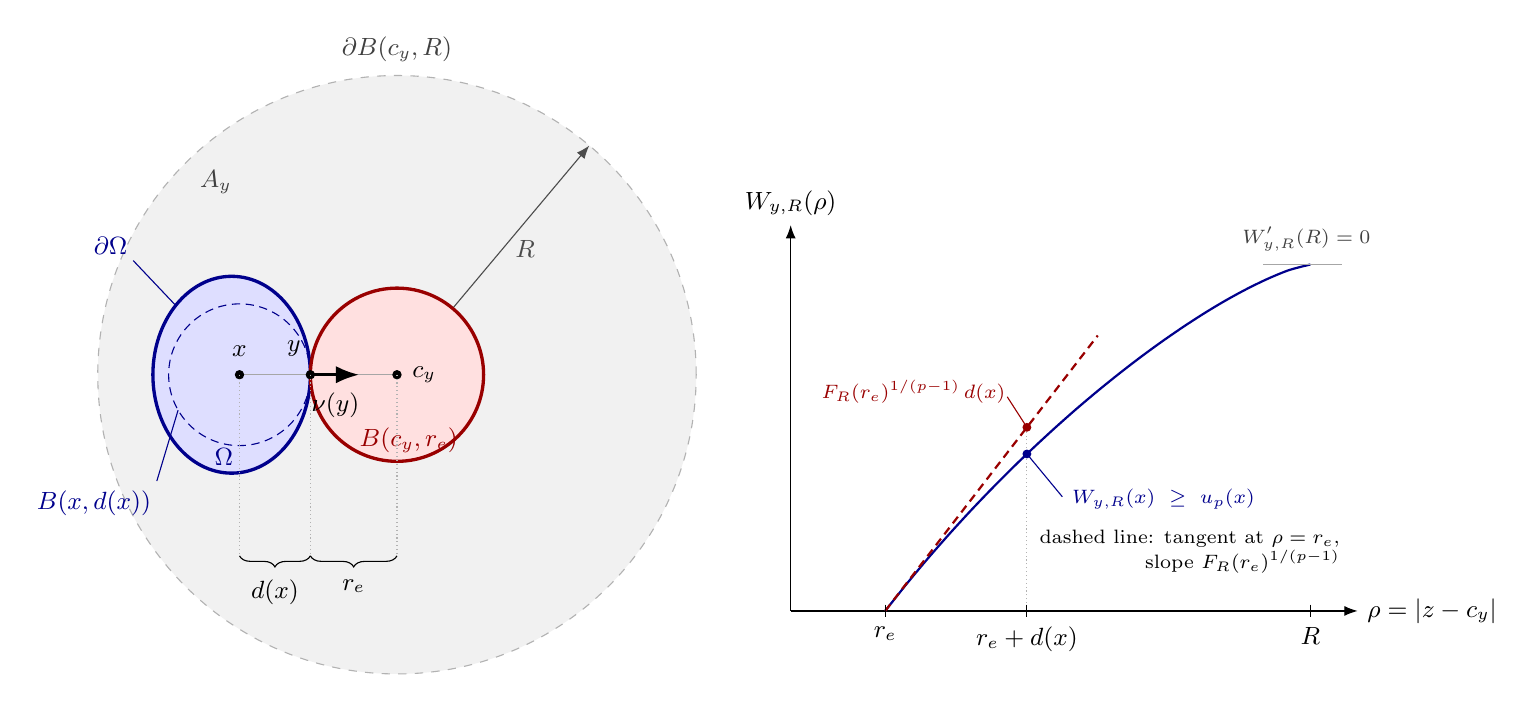
\begin{tikzpicture}[scale=1,>=Latex,every node/.style={font=\small}]
  % ================= left panel: geometry =================
  \coordinate (c) at (0,0);        % centre of the exterior ball
  \coordinate (y) at (-1.1,0);     % tangency point on the boundary
  \coordinate (x) at (-2.0,0);     % interior point with d(x)=0.9
  % containing annulus and auxiliary sphere
  \fill[gray!11,even odd rule] (c) circle (3.8) (c) circle (1.1);
  \draw[dashed,gray!60] (c) circle (3.8);
  \node[gray!50!black,anchor=south] at (0,3.85) {$\partial B(c_y,R)$};
  \node[gray!50!black] at (-2.3,2.45) {$A_y$};
  \draw[->,gray!60!black] (c) -- (50:3.8) node[pos=0.55,right=1pt] {$R$};
  % domain
  \fill[blue!13] (-2.1,0) ellipse (1.0 and 1.25);
  \draw[very thick,blue!55!black] (-2.1,0) ellipse (1.0 and 1.25);
  \node[blue!55!black] at (-2.2,-1.05) {$\Omega$};
  \draw[blue!55!black,thin] (-3.35,1.45) -- (-2.81,0.88);
  \node[blue!55!black,anchor=south east] at (-3.3,1.4) {$\partial\Omega$};
  % inscribed ball
  \draw[densely dashed,blue!55!black] (x) circle (0.9);
  \draw[blue!55!black,thin] (-3.05,-1.35) -- (-2.78,-0.45);
  \node[blue!55!black,anchor=north east] at (-3.0,-1.35) {$B(x,d(x))$};
  % exterior ball
  \fill[red!12] (c) circle (1.1);
  \draw[very thick,red!60!black] (c) circle (1.1);
  \node[red!60!black,anchor=north] at (0.15,-0.55) {$B(c_y,r_e)$};
  % collinear points, normal
  \draw[gray!70,thin] (x) -- (c);
  \draw[->,very thick] (y) -- ++(0.62,0);
  \node[anchor=north] at (-0.78,-0.1) {$\nu(y)$};
  \fill (c) circle (1.7pt) node[anchor=west,xshift=2pt] {$c_y$};
  \fill (y) circle (1.7pt) node[anchor=south,xshift=-6pt,yshift=3pt] {$y$};
  \fill (x) circle (1.7pt) node[above=3pt] {$x$};
  % distances
  \draw[gray!60,densely dotted] (x) -- (-2.0,-2.3);
  \draw[gray!60,densely dotted] (y) -- (-1.1,-2.3);
  \draw[gray!60,densely dotted] (c) -- (0,-2.3);
  \draw[decorate,decoration={brace,mirror,amplitude=4pt}] (-2.0,-2.3) -- (-1.1,-2.3)
     node[midway,below=5pt] {$d(x)$};
  \draw[decorate,decoration={brace,mirror,amplitude=4pt}] (-1.1,-2.3) -- (0,-2.3)
     node[midway,below=5pt] {$r_e$};
  % ================= right panel: radial profile =================
  \begin{scope}[shift={(5.0,-3.0)}]
    \draw[->] (0,0) -- (7.2,0) node[right] {$\rho=\abs{z-c_y}$};
    \draw[->] (0,0) -- (0,4.9) node[above] {$W_{y,R}(\rho)$};
    \draw[thick,blue!55!black] plot[smooth] coordinates
      {(1.200,0.000) (1.470,0.340) (1.740,0.664) (2.010,0.972) (2.280,1.267)
       (2.550,1.549) (2.820,1.820) (3.090,2.079) (3.360,2.328) (3.630,2.567)
       (3.900,2.795) (4.170,3.013) (4.440,3.221) (4.710,3.418) (4.980,3.604)
       (5.250,3.779) (5.520,3.941) (5.790,4.088) (6.060,4.219) (6.330,4.329)
       (6.600,4.400)};
    % tangent at r_e
    \draw[red!60!black,thick,densely dashed] (1.2,0) -- (3.9,3.498);
    \node[anchor=east,align=right,font=\scriptsize] at (7.1,0.75)
      {dashed line: tangent at $\rho=r_e$,\\ slope $F_R(r_e)^{1/(p-1)}$};
    % horizontal tangent at R
    \draw[gray!70] (6.0,4.40) -- (7.0,4.40);
    \node[gray!50!black,anchor=south,font=\scriptsize] at (6.55,4.44) {$W_{y,R}'(R)=0$};
    % point rho = r_e + d(x)
    \draw[gray!60,densely dotted] (3.0,0) -- (3.0,2.332);
    \fill[blue!55!black] (3.0,1.994) circle (1.6pt);
    \fill[red!60!black]  (3.0,2.332) circle (1.6pt);
    \draw[blue!55!black,thin] (3.0,1.994) -- (3.45,1.45);
    \node[blue!55!black,anchor=west,font=\scriptsize] at (3.45,1.42) {$W_{y,R}(x)\ \ge\ u_p(x)$};
    \draw[red!60!black,thin] (3.0,2.332) -- (2.75,2.72);
    \node[red!60!black,anchor=east,font=\scriptsize] at (2.85,2.78) {$F_R(r_e)^{1/(p-1)}\,d(x)$};
    % ticks
    \foreach \xx/\lab in {1.2/$r_e$, 3.0/$r_e+d(x)$, 6.6/$R$}
      {\draw (\xx,0.08) -- (\xx,-0.08) node[below] {\lab};}
  \end{scope}
\end{tikzpicture}}
\caption{Left: the exterior-barrier geometry. The exterior ball $B(c_y,r_e)$ (red) touches
$\partial\Omega$ at $y$ and is disjoint from $\Omega$ (blue). For a point $x$ whose nearest
boundary point is $y$, the inscribed ball $B(x,d(x))$ (dashed) touches the exterior ball at
the same point, so $x$, $y$ and $c_y$ are collinear and $\abs{x-c_y}=r_e+d(x)$, which is the
tangency identity \eqref{eq:tangency}. The ball $B(c_y,R)$ with $R>D+r_e$ contains
$\Omega$, and the barrier is defined on the shaded annulus $A_y=\{r_e<\abs{z-c_y}<R\}$.
Right: the radial profile $W_{y,R}$ of \eqref{eq:W}, computed for $n=2$, $p=4$, $r_e=1$,
$R=4$. It vanishes at $\rho=r_e$, is concave because $F_R$ is decreasing, and has zero slope
at $\rho=R$; it therefore lies below its tangent at $r_e$, and reading the picture at
$\rho=r_e+d(x)$ gives $u_p(x)\le W_{y,R}(x)\le F_R(r_e)^{1/(p-1)}d(x)$, which is
Proposition~\ref{thm:upper}.}
\label{fig:exterior-annulus}
\end{figure}

\begin{proof}
Figure~\ref{fig:exterior-annulus} summarizes the geometry. For $z\in\Omega$ we
have $\abs{z-c_y}>r_e$, as noted after Definition~\ref{def:ext-ball}, and
$\abs{z-c_y}\le\abs{z-y}+r_e\le D+r_e<R$, so $\Omega\subset A_y$. Writing
$\rho=\abs{z-c_y}$, the radial derivative is
$W_{y,R}'(\rho)=F_R(\rho)^{1/(p-1)}\ge0$, hence
$\rho^{n-1}\abs{W_{y,R}'}^{p-2}W_{y,R}'=(R^n-\rho^n)/n$, whose derivative is
$-\rho^{n-1}$. Therefore $-\Delta_pW_{y,R}=1$ in $A_y$, and
$W_{y,R}\in C^1(\overline{A_y})$ since $F_R^{1/(p-1)}$ is continuous on
$[r_e,R]$. Its restriction to $\Omega$ is a non-negative function in
$W^{1,\infty}(\Omega)$ satisfying \eqref{eq:supersol} with equality, so
Lemma~\ref{lem:comparison}(i) gives $u_p\le W_{y,R}$ in $\Omega$.
\end{proof}

Anchoring the barrier at a nearest boundary point identifies its radial
increment with $d(x)$.
\begin{proposition}[Exterior-ball upper estimate]\label{thm:upper}
Let $\Omega\subset\R^n$ be a bounded domain satisfying
Definition~\ref{def:ext-ball} with radius $r_e>0$, and let $K_\Omega$,
$K_\Omega^+$ be as in \eqref{eq:Komega}. Then, for every $p>1$,
\[
u_p(x)\ \le\ K_\Omega^{1/(p-1)}\,d(x)
\qquad\text{for every }x\in\Omega,
\]
and consequently
$u_p\le d+4\rho_\Omega\log K_\Omega^+/p$ in $\Omega$ for every
$p\ge\max\{2,\,1+\log K_\Omega^+\}$.
\end{proposition}
\begin{proof}
Fix $x\in\Omega$ and choose $y\in\partial\Omega$ with $\abs{x-y}=d(x)$. By
\eqref{eq:tangency}, $\abs{x-c_y}=r_e+d(x)$. Let $R>D+r_e$. By
Lemma~\ref{lem:barrier} and \eqref{eq:F-decreasing},
\[
u_p(x)\ \le\ W_{y,R}(x)
=\int_{r_e}^{r_e+d(x)}F_R(s)^{1/(p-1)}\,ds
\ \le\ F_R(r_e)^{1/(p-1)}\,d(x).
\]
Letting $R\downarrow D+r_e$ gives $F_R(r_e)\to K_\Omega$ and hence
$u_p(x)\le K_\Omega^{1/(p-1)}d(x)$. The second assertion follows from
$K_\Omega^{1/(p-1)}\le (K_\Omega^+)^{1/(p-1)}\le1+4\log K_\Omega^+/p$
(Lemma~\ref{lem:elementary}(ii)) and $d\le\rho_\Omega$.
\end{proof}

\begin{proof}[Proof of Theorem~\ref{thm:main}]
The two-sided bound \eqref{eq:main-pointwise} is
Lemma~\ref{lem:ball-comparison} together with Proposition~\ref{thm:upper},
and \eqref{eq:main-rate} follows from the second assertion of
Proposition~\ref{thm:upper} and Proposition~\ref{thm:lower}.
\end{proof}

\begin{remark}[Scaling]\label{rem:scaling}
For $a>0$ and $\Omega_a:=a\Omega$ one has
$u_{p,\Omega_a}(ax)=a^{\gamma}u_{p,\Omega}(x)$,
$d_{\Omega_a}(ax)=a\,d_\Omega(x)$ and $K_{\Omega_a}=a\,K_\Omega$, so the
multiplicative estimate $u_p\le K_\Omega^{1/(p-1)}d$ is exactly invariant
under dilation, since $a^{1/(p-1)}\cdot a=a^{\gamma}$. The additive
first-order constant in \eqref{eq:main-rate}, by contrast, changes by a
logarithm of the scale; this is intrinsic to the $p\to\infty$ expansion
rather than a defect of the estimate. Its dependence on $r_e$ is also
explicit: for fixed $D$ and $n\ge2$, $K_\Omega\sim D^nr_e^{\,1-n}/n$ as
$r_e\downarrow0$, so the constant grows logarithmically in $1/r_e$, whereas
the constant in Theorem~\ref{thm:universal-rate} is independent of $r_e$.
\end{remark}

\subsection{Convex domains}\label{subsec:convex}
Every bounded convex domain admits every $r_e>0$ as an exterior radius, and
expanding \eqref{eq:Komega} binomially,
\begin{equation}\label{eq:K-expansion}
K_\Omega(r_e)=\frac1n\sum_{m=1}^{n}\binom nm D^{\,m}\,r_e^{\,1-m}
\ \downarrow\ D
\qquad\text{as }r_e\uparrow\infty .
\end{equation}
Letting $r_e\to\infty$ in Proposition~\ref{thm:upper} therefore gives the
following estimate, in which only the diameter enters and no boundary
regularity is assumed; it is the estimate one would obtain directly by
comparing with the one-dimensional profile of a supporting slab.
\begin{corollary}[Convex domains]\label{cor:convex}
Let $\Omega\subset\R^n$ be a bounded open convex set and $D^+:=\max\{1,D\}$.
Then, for every $p>1$,
\begin{equation}\label{eq:slab}
u_p(x)\ \le\ D^{1/(p-1)}\,d(x)
\qquad\text{for every }x\in\Omega,
\end{equation}
and
$\norm{u_p-d}_{L^\infty(\Omega)}\le\bigl(4\rho_\Omega\log D^+ + C(n,\rho_\Omega)\bigr)/p$
for every $p\ge\max\{2,1+\log D^+\}$.
\end{corollary}
\begin{proof}
For each $r_e>0$, Proposition~\ref{thm:upper} gives
$u_p\le K_\Omega(r_e)^{1/(p-1)}d$; let $r_e\to\infty$ and use
\eqref{eq:K-expansion}. The additive bound follows from
Lemma~\ref{lem:elementary}(ii) with $K=D^+$ and Proposition~\ref{thm:lower}.
\end{proof}

\subsection{A distance-function supersolution}\label{subsec:dbarrier}
When the distance function is strictly superharmonic in the distributional
sense, a scalar multiple of $d$ is itself a supersolution. On the domains
where this applies it gives a sharper constant than the exterior annulus.
\begin{theorem}[Distance supersolution estimate]\label{thm:dbarrier}
Let $\Omega\subset\R^n$ be a bounded domain and suppose there is $\lambda>0$
with
\begin{equation}\label{eq:kappa}
-\Delta d\ \ge\ \lambda
\qquad\text{in }\mathcal D'(\Omega),
\end{equation}
that is,
$\int_\Omega\nabla d\cdot\nabla\varphi\,dx\ge\lambda\int_\Omega\varphi\,dx$ for
every non-negative $\varphi\in C_c^\infty(\Omega)$. Then, for every $p>1$,
\begin{equation}\label{eq:dbarrier-pointwise}
u_p(x)\ \le\ \lambda^{-1/(p-1)}\,d(x)
\qquad\text{for every }x\in\Omega.
\end{equation}
In particular $u_p\le d$ for every $p>1$ if $\lambda\ge1$, while if
$\lambda<1$ then $u_p\le d+4\rho_\Omega\log(1/\lambda)/p$ in $\Omega$ for
every $p\ge\max\{2,\,1+\log(1/\lambda)\}$.
\end{theorem}
\begin{proof}
Set $\theta:=\lambda^{-1/(p-1)}$ and $w:=\theta d$. By
Lemma~\ref{lem:d-in-W1p}, $w\in W^{1,\infty}(\Omega)$, $w\ge0$, and
$\abs{\nabla d}=1$ almost everywhere, so for every non-negative
$\varphi\in C_c^\infty(\Omega)$,
\[
\int_\Omega\abs{\nabla w}^{p-2}\nabla w\cdot\nabla\varphi\,dx
=\theta^{p-1}\int_\Omega\nabla d\cdot\nabla\varphi\,dx
\ \ge\ \theta^{p-1}\lambda\int_\Omega\varphi\,dx
=\int_\Omega\varphi\,dx .
\]
Lemma~\ref{lem:comparison}(i) gives \eqref{eq:dbarrier-pointwise}. If
$\lambda\ge1$ then $\theta\le1$. If $\lambda<1$,
Lemma~\ref{lem:elementary}(ii) with $K:=1/\lambda>1$ gives
$\theta\le1+4\log(1/\lambda)/p$ for $p\ge\max\{2,1+\log(1/\lambda)\}$, and
$d\le\rho_\Omega$.
\end{proof}

\begin{remark}\label{rem:dbarrier-structure}
Estimate \eqref{eq:dbarrier-pointwise} has the form of
\eqref{eq:main-pointwise} and \eqref{eq:slab} with $K_\Omega$, respectively
$D$, replaced by $1/\lambda$; it is invariant under dilation in the sense of
Remark~\ref{rem:scaling}, since $\lambda$ scales like the inverse of a length.
On the unit ball with $n\ge2$, Proposition~\ref{prop:umc} gives
$\lambda=n-1\ge1$, and the conclusion $u_p\le d$ is the inequality obtained
directly in Theorem~\ref{thm:ball}, whereas Corollary~\ref{cor:convex} only
gives $u_p\le 2^{1/(p-1)}d$ there.
\end{remark}

The hypothesis \eqref{eq:kappa} is a curvature condition. Principal
curvatures $\kappa_1,\dots,\kappa_{n-1}$ of a $C^2$ boundary are taken with
respect to the outer unit normal and signed so that spheres have positive
curvature, and $H:=\sum_i\kappa_i$ is the non-averaged mean curvature. In these
conventions, Lewis--Li--Li \cite[Theorem~1.6 and Proposition~3.9]{LewisLiLi2012}
give the following.
\begin{proposition}[Uniform mean-convexity criterion of Lewis--Li--Li]\label{prop:umc}
Let $n\ge2$ and let $\Omega\subset\R^n$ be a bounded $C^2$ domain with
$H\ge H_0>0$ on $\partial\Omega$. Then $-\Delta d\ge H_0$ in
$\mathcal D'(\Omega)$. In particular this holds if $\Omega$ is uniformly
convex, $\kappa_i\ge\kappa_0>0$ for every $i$, with $H_0=(n-1)\kappa_0$.
\end{proposition}

For orientation we recall the mechanism, which is contained in the
distance-function theory of Crasta--Malusa~\cite{CrastaMalusa},
Mantegazza--Mennucci~\cite{MM}, Li--Nirenberg~\cite{LiNir}, and
Cannarsa--Sinestrari~\cite[Ch.~3]{CS}. For a bounded $C^2$ domain, $d$ is
locally semiconcave, so $-\Delta d$ is a locally finite signed Radon measure
whose singular part, carried by the cut locus of $\partial\Omega$ (a Lebesgue
null set), is non-negative; off the cut locus $d$ is $C^2$ and
\begin{equation}\label{eq:reg-set-formula}
-\Delta d(x)=\sum_{i=1}^{n-1}\frac{\kappa_i(y(x))}{1-d(x)\,\kappa_i(y(x))}
\ \ge\ H(y(x)),
\end{equation}
where $y(x)$ is the nearest boundary point, every denominator is positive, and
the inequality follows from
$\frac{\kappa_i}{1-t\kappa_i}-\kappa_i=\frac{t\kappa_i^2}{1-t\kappa_i}\ge0$.
Hence the absolutely continuous part of $-\Delta d$ has density at least
$H_0$ and the singular part is non-negative, which is $-\Delta d\ge H_0$ in
$\mathcal D'(\Omega)$.

\begin{remark}\label{rem:LLL}
Lewis, Li and Li~\cite[Theorem~1.7]{LewisLiLi2012} proved that, for a bounded
$C^2$ domain, $-\Delta d\ge0$ in $\mathcal D'(\Omega)$ if and only if
$\partial\Omega$ is weakly mean convex. Strict positivity in \eqref{eq:kappa}
is exactly what the barrier requires: $\theta d$ is a weak supersolution of
$-\Delta_pw=1$ if and only if $-\Delta d\ge\theta^{1-p}$ in
$\mathcal D'(\Omega)$, so if \eqref{eq:kappa} holds for no $\lambda>0$ then no
positive multiple of $d$ serves as a barrier. Uniform mean convexity cannot be
weakened to strict convexity: the boundary of $\{\sum_ix_i^4<1\}$ is strictly
convex but all its principal curvatures vanish where it meets a coordinate
axis, so $\inf_{\partial\Omega}H=0$. Convexity alone is not enough either: on
a rectangular box $-\Delta d$ is purely singular, concentrated on the ridge
set, and no $\lambda>0$ is admissible. Corollary~\ref{cor:convex} and
Theorem~\ref{thm:dbarrier} therefore apply under distinct, non-equivalent
hypotheses.
\end{remark}

%%%%%%%%%%%%%%%%%%%%%%%%%%%%%%%%%%%%%%%%%%%%%%%%%%%%%%%%%%%%%%%%%%%%%%%%%%%%%
\section{The gradient bound}\label{sec:gradient-bound}
%%%%%%%%%%%%%%%%%%%%%%%%%%%%%%%%%%%%%%%%%%%%%%%%%%%%%%%%%%%%%%%%%%%%%%%%%%%%%
The gradient maximum principle of Payne--Philippin~\cite{PP},
Sperb~\cite{Sperb}, and Kawohl~\cite{Kaw1987}, the last devoted specifically
to the location of gradient maxima for quasilinear problems, reduces the
global gradient bound to a boundary estimate; Mariconda and Treu~\cite{MT}
prove a gradient maximum principle for minima of convex integral functionals
under minimal hypotheses. The lemma below is therefore not new; for
completeness we give a proof adapted to the degenerate $p$-Laplacian, by
differentiating the equation on the noncritical set. What matters for us is
that it holds without any hypothesis on the sign of the boundary curvature and
with no constant depending on $p$.
\begin{lemma}[Gradient maximum principle]\label{lem:grad-max}
Let $\Omega\subset\R^n$ be a bounded $C^2$ domain and $p>1$. Then
\begin{equation}\label{eq:grad-max}
\max_{\overline\Omega}\abs{\nabla u_p}=\max_{\partial\Omega}\abs{\nabla u_p}.
\end{equation}
\end{lemma}
\begin{proof}
The maximum is attained because $u_p\in C^{1}(\overline\Omega)$, and $L_p>0$
because $u_p\not\equiv0$. Suppose the maximum is attained at an interior
point $x_0$.
Then $\nabla u_p(x_0)\ne0$, so there is a connected open $V\ni x_0$ with
$V\Subset\Omega$ on which $\abs{\nabla u_p}$ is bounded away from $0$; on $V$
the equation is uniformly elliptic with smooth dependence on $\nabla u_p$ and
$u_p\in C^\infty(V)$. Write $A(\xi):=\abs{\xi}^{p-2}\xi$ and
\[
a_{ij}:=\frac{\partial A_i}{\partial\xi_j}(\nabla u_p)
=\abs{\nabla u_p}^{p-2}
\Bigl(\delta_{ij}+(p-2)\frac{(u_p)_i(u_p)_j}{\abs{\nabla u_p}^{2}}\Bigr),
\]
a symmetric matrix with eigenvalues $\abs{\nabla u_p}^{p-2}$ and
$(p-1)\abs{\nabla u_p}^{p-2}$, hence uniformly positive definite on compact
subsets of $V$ for every $p>1$. Differentiating
$\partial_iA_i(\nabla u_p)=-1$ with respect to $x_k$ gives
\begin{equation}\label{eq:diff-eq}
\partial_i\bigl(a_{ij}(u_p)_{jk}\bigr)=0
\qquad\text{in }V,\ k=1,\dots,n.
\end{equation}
Put $v:=\tfrac12\abs{\nabla u_p}^2$, so $v_j=\sum_k(u_p)_k(u_p)_{kj}$. Using
\eqref{eq:diff-eq},
\begin{equation}\label{eq:subsolution}
\partial_i\bigl(a_{ij}v_j\bigr)
=\sum_k\Bigl[(u_p)_k\,\partial_i\bigl(a_{ij}(u_p)_{kj}\bigr)
+a_{ij}(u_p)_{ki}(u_p)_{kj}\Bigr]
=\sum_ka_{ij}(u_p)_{ki}(u_p)_{kj}\ \ge\ 0
\end{equation}
in $V$. Thus $v$ is a subsolution in $V$ of a linear divergence-form uniformly
elliptic operator without zeroth-order term, and it attains at $x_0\in V$ its
maximum over $V$. By the strong maximum principle \cite[Theorem~8.19]{GT},
$v$ is constant on $V$. Then the left-hand side of \eqref{eq:subsolution}
vanishes, so $a_{ij}(u_p)_{ki}(u_p)_{kj}=0$ for every $k$, and positive
definiteness forces $D^2u_p=0$ on $V$. But then
$\Delta_pu_p=a_{ij}(u_p)_{ij}=0$ on $V$, contradicting $-\Delta_pu_p=1$.
For $p=2$ the argument is the classical observation that
$\Delta\abs{\nabla u}^2=2\abs{D^2u}^2\ge0$ when $\Delta u$ is constant;
localizing in $\{\abs{\nabla u_p}>0\}$ is what avoids the degeneracy of the
$p$-Laplacian at critical points.
\end{proof}

The exterior barrier agrees with the boundary datum at the tangency point, so
its inward normal derivative bounds that of $u_p$.
\begin{lemma}[Boundary gradient estimate]\label{lem:boundary-gradient}
Let $\Omega\subset\R^n$ be a bounded $C^2$ domain with uniform exterior ball
radius $r_e>0$. Then, for every $p>1$ and every $y\in\partial\Omega$,
$\abs{\nabla u_p(y)}^{\,p-1}\le K_\Omega$.
\end{lemma}
\begin{proof}
Let $R>D+r_e$ and keep the notation of Lemma~\ref{lem:barrier}. Let
$\tau:=-\nu(y)$ be the inward unit normal. For small $t>0$ the point $y+t\tau$
lies in $\Omega$ with $\abs{y+t\tau-c_y}=r_e+t$, and $u_p(y)=W_{y,R}(y)=0$, so
\[
\frac{u_p(y+t\tau)}{t}\ \le\ \frac{W_{y,R}(y+t\tau)}{t}
=\frac1t\int_{r_e}^{r_e+t}F_R(s)^{1/(p-1)}\,ds.
\]
Letting $t\downarrow0$ and using $u_p\in C^1(\overline\Omega)$ together with
the continuity of $F_R$ gives $\partial_\tau u_p(y)\le F_R(r_e)^{1/(p-1)}$.
Because $u_p$ vanishes on $\partial\Omega$ its tangential derivatives vanish
there, and $u_p\ge0$ gives $\partial_\tau u_p(y)\ge0$; hence
$\abs{\nabla u_p(y)}=\partial_\tau u_p(y)\le F_R(r_e)^{1/(p-1)}$. Let
$R\downarrow D+r_e$.
\end{proof}
\begin{proof}[Proof of Theorem~\ref{thm:gradient-bound}]
Combine Lemma~\ref{lem:grad-max} with Lemma~\ref{lem:boundary-gradient}.
\end{proof}

\begin{remark}\label{rem:1d}
For $n=1$ and $\Omega=(0,L)$, put $a:=L/2$. Integrating the equation once and
using $u_p'(a)=0$ gives $\abs{u_p'}^{p-2}u_p'=a-t$, so
$u_p(t)=\frac{p-1}{p}\bigl(a^{\gamma}-\abs{t-a}^{\gamma}\bigr)$ and
$\norm{u_p'}_{L^\infty(0,L)}^{\,p-1}=a=L/2$, whereas $D=L$ and
$K_\Omega=L$ for every choice of $r_e$. Thus \eqref{eq:gradient-bound} holds
in dimension one with room to spare.
\end{remark}

Theorem~\ref{thm:gradient-bound}, Lemma~\ref{lem:segment}, and the uniform
convergence of $u_p$ determine the limit of the gradient supremum; that this
limit is $1$ does not imply uniform convergence of $\nabla u_p$ to $\nabla d$,
see Proposition~\ref{prop:ball-gradient}.
\begin{corollary}[Limit of the gradient supremum]\label{cor:gradient-limit}
Let $\Omega$ be a bounded $C^2$ domain. Then
$\norm{\nabla u_p}_{L^\infty(\Omega)}\to1$ as $p\to\infty$.
\end{corollary}
\begin{proof}
Theorem~\ref{thm:gradient-bound} gives
$\limsup_pL_p\le\lim_p(K_\Omega^+)^{1/(p-1)}=1$. Conversely, fix $x_0$ with
$d(x_0)=\rho_\Omega$; Lemma~\ref{lem:segment} gives
$L_p\ge u_p(x_0)/\rho_\Omega$, and $u_p(x_0)\to\rho_\Omega$ by
Theorem~\ref{thm:universal-rate}.
\end{proof}

%%%%%%%%%%%%%%%%%%%%%%%%%%%%%%%%%%%%%%%%%%%%%%%%%%%%%%%%%%%%%%%%%%%%%%%%%%%%%
\section{Consequences for related quantities}\label{sec:consequences}
%%%%%%%%%%%%%%%%%%%%%%%%%%%%%%%%%%%%%%%%%%%%%%%%%%%%%%%%%%%%%%%%%%%%%%%%%%%%%
Some of the literature works with the normalized torsion function
$v_p:=u_p/k_p$, $k_p:=\norm{\nabla u_p}_{L^p(\Omega)}$, for which
$\norm{\nabla v_p}_{L^p(\Omega)}=1$ and $-\Delta_pv_p=k_p^{1-p}$. The
mean-to-max ratio of the $p$-torsion function, studied by Briani and
Bucur~\cite{BB} in connection with honeycomb structures, is
\[
\Phi_p(\Omega):=\frac{1}{\abs{\Omega}\,\norm{u_p}_{L^\infty(\Omega)}}
\int_\Omega u_p\,dx,
\qquad
\Phi_\infty(\Omega):=\frac{1}{\abs{\Omega}\,\rho_\Omega}\int_\Omega d\,dx.
\]
\begin{corollary}[Normalized torsion and mean-to-max ratio]\label{cor:consequences}
Suppose $\norm{u_p-d}_{L^\infty(\Omega)}\le C_1/p$ for all $p\ge p_1$. Then
there are $p_2=p_2(\Omega,C_1,p_1)$ and $C=C(\Omega,C_1)>0$ such that, for
all $p\ge p_2$,
\[
\norm{v_p-d}_{L^\infty(\Omega)}\le\frac{C}{p},
\qquad
\abs{\Phi_p(\Omega)-\Phi_\infty(\Omega)}\le\frac{C}{p}.
\]
With $C_1$ and $p_1$ from Theorem~\ref{thm:universal-rate}, $p_2$ and $C$
depend only on $n$ and $\Omega$.
\end{corollary}
\begin{proof}
Testing \eqref{eq:weak} with $u_p$ gives $k_p^p=\int_\Omega u_p>0$. Put
$I:=\int_\Omega d>0$ and
\[
p_2:=\max\Bigl\{p_1,\ \frac{2C_1\abs\Omega}{I},\ \frac{2C_1}{\rho_\Omega}\Bigr\}.
\]
For $p\ge p_2$ the hypothesis gives $\tfrac12I\le\int_\Omega u_p\le2I$ and
$\norm{u_p}_{L^\infty}\ge\rho_\Omega/2$, hence
$\abs{\log k_p}=\frac1p\abs{\log\int_\Omega u_p}\le C/p$ and
$\abs{k_p^{-1}-1}\le C/p$. Since $\norm{u_p}_{L^\infty}\le\rho_\Omega+C_1/p$,
\[
\norm{v_p-d}_\infty\le\abs{k_p^{-1}-1}\norm{u_p}_\infty
+\norm{u_p-d}_\infty\le\frac{C}{p}.
\]
For the ratio, write $\Phi_p=m_p/M_p$ and $\Phi_\infty=m_\infty/M_\infty$
with $m_p:=\abs{\Omega}^{-1}\int_\Omega u_p$, $M_p:=\norm{u_p}_\infty$,
$m_\infty:=\abs{\Omega}^{-1}\int_\Omega d$ and $M_\infty:=\rho_\Omega$. Then
$\abs{m_p-m_\infty}\le C_1/p$, $\abs{M_p-M_\infty}\le C_1/p$,
$M_p\ge\rho_\Omega/2$ for $p\ge p_2$, and $m_\infty\le M_\infty$, so
\[
\abs{\Phi_p-\Phi_\infty}
\le\frac{\abs{m_p-m_\infty}}{M_p}
+m_\infty\frac{\abs{M_p-M_\infty}}{M_pM_\infty}
\le\frac{4C_1}{\rho_\Omega\,p}. \qedhere
\]
\end{proof}

%%%%%%%%%%%%%%%%%%%%%%%%%%%%%%%%%%%%%%%%%%%%%%%%%%%%%%%%%%%%%%%%%%%%%%%%%%%%%
\section{Quantitative convergence of the gradients}\label{sec:gradients}
%%%%%%%%%%%%%%%%%%%%%%%%%%%%%%%%%%%%%%%%%%%%%%%%%%%%%%%%%%%%%%%%%%%%%%%%%%%%%
The estimates of this section quantify the strong $L^q$ convergence of
$\nabla u_p$ proved in~\cite{BLR} by combining the uniform error of
Theorem~\ref{thm:universal-rate} with the finite-measure structure of
$-\Delta d$ from Lemma~\ref{lem:tv-exterior-ball}. The following monotonicity
inequality converts the energy defect into an $L^2$ gradient defect, using
$\abs{\nabla d}=1$ almost everywhere.
\begin{lemma}\label{lem:monotonicity}
Let $p\ge2$, $\xi\in\R^n$ and $\abs{\eta}=1$. Then
\begin{equation}\label{eq:monotonicity}
\bigl(\abs{\xi}^{p-2}\xi-\eta\bigr)\cdot(\xi-\eta)
\ \ge\ \tfrac12\abs{\xi-\eta}^{2}.
\end{equation}
\end{lemma}
\begin{proof}
For $\xi=0$ the left-hand side equals $1$ and the right-hand side $1/2$, so
assume $r:=\abs{\xi}>0$ and put $c:=(\xi\cdot\eta)/r\in[-1,1]$. Twice the
left-hand side minus $\abs{\xi-\eta}^2$ equals $2r^p+1-r^2-2r^{p-1}c$, which
is minimized over $c\in[-1,1]$ at $c=1$, where it equals
$2r^p-2r^{p-1}+1-r^2=(r-1)\bigl(2r^{p-1}-r-1\bigr)$. For $r\ge1$ we have
$r^{p-1}\ge r$, so both factors are non-negative; for $0<r\le1$ we have
$r^{p-1}\le r$, so both are non-positive. In either case the product is
non-negative.
\end{proof}

\begin{theorem}[Quantitative gradient convergence]\label{thm:gradient-rate}
Let $\Omega\subset\R^n$ be a bounded domain such that $\mu:=-\Delta d$
is a signed Radon measure on $\Omega$ with $\abs{\mu}(\Omega)<\infty$. Then,
for all sufficiently large $p$,
\begin{equation}\label{eq:L2-rate}
\norm{\nabla u_p-\nabla d}_{L^2(\Omega)}\ \le\ \frac{C}{\sqrt p},
\qquad C=C\bigl(n,D,\abs\Omega,\abs\mu(\Omega)\bigr),
\end{equation}
and consequently
$\norm{\nabla u_p-\nabla d}_{L^q(\Omega)}\le C\abs\Omega^{1/q-1/2}p^{-1/2}$ for
each $q\in[1,2]$. For each fixed $q\in[2,\infty)$ there exist
$p_q=p_q(n,D,q)>\max\{n,q\}$ and $C_q=C_q(n,D,\abs\Omega,\abs\mu(\Omega))$
such that, for every $p\ge p_q$,
\begin{equation}\label{eq:Lq-rate}
\norm{\nabla u_p-\nabla d}_{L^q(\Omega)}\ \le\ C_q\,p^{-1/q}.
\end{equation}
In particular, by Lemma~\ref{lem:tv-exterior-ball}, these conclusions hold on
every bounded $C^1$ domain satisfying \eqref{eq:ext-ball}, and hence on every
bounded $C^2$ domain.
\end{theorem}
\begin{proof}
Take $p>\max\{n,2\}$ and put $e_p:=u_p-d$. By Lemma~\ref{lem:d-in-W1p},
$e_p\in W^{1,p}_0(\Omega)$; since $p>n$, its extension by zero to $\R^n$ is
continuous by the Morrey embedding. Testing \eqref{eq:weak} with $e_p$,
\begin{equation}\label{eq:test1}
\int_\Omega\abs{\nabla u_p}^{p-2}\nabla u_p\cdot\nabla e_p\,dx
=\int_\Omega e_p\,dx.
\end{equation}
Since $\abs{\nabla d}=1$ almost everywhere,
$\abs{\nabla d}^{p-2}\nabla d=\nabla d$, and the finite-measure hypothesis
gives
\begin{equation}\label{eq:test2}
\int_\Omega\nabla d\cdot\nabla e_p\,dx=\int_\Omega e_p\,d\mu .
\end{equation}
Identity \eqref{eq:test2} holds by definition for $e_p\in C_c^\infty(\Omega)$;
for general $e_p$, approximate in $W^{1,p}_0(\Omega)$ by functions in
$C_c^\infty(\Omega)$, extend the approximants by zero to $\R^n$, and apply the
Morrey embedding there; since $p>n$ this gives uniform convergence as well, so
both the Lebesgue integral and the pairing against the finite measure $\mu$
pass to the limit. Subtracting \eqref{eq:test2} from \eqref{eq:test1},
\[
I_p:=\int_\Omega
\bigl(\abs{\nabla u_p}^{p-2}\nabla u_p-\nabla d\bigr)\cdot
\bigl(\nabla u_p-\nabla d\bigr)\,dx
=\int_\Omega e_p\,dx-\int_\Omega e_p\,d\mu ,
\]
and $I_p\ge0$ by Lemma~\ref{lem:monotonicity}. Theorem~\ref{thm:universal-rate}
gives
\[
0\ \le\ I_p\ \le\ \bigl(\abs{\Omega}+\abs{\mu}(\Omega)\bigr)
\norm{e_p}_{L^\infty(\Omega)}\ \le\ \frac{C(n,D)\bigl(\abs{\Omega}+\abs{\mu}(\Omega)\bigr)}{p}.
\]
Applying \eqref{eq:monotonicity} pointwise with $\xi=\nabla u_p$ and
$\eta=\nabla d$ gives $\tfrac12\norm{\nabla u_p-\nabla d}_{L^2}^2\le I_p$,
which is \eqref{eq:L2-rate}; for $1\le q\le2$, H\"older's inequality gives
the stated bound.

Fix $q\ge2$ and take $p\ge q$. Write $h_p:=\abs{\nabla u_p-\nabla d}$ and
$E_p:=\{\abs{\nabla u_p}>2\}$. On $\Omega\setminus E_p$ one has $h_p\le3$;
on $E_p$ one has $h_p\le\tfrac32\abs{\nabla u_p}$ and
$\abs{\nabla u_p}^q\le2^{q-p}\abs{\nabla u_p}^p$. Hence
\[
\int_\Omega h_p^q\,dx
\le 3^{q-2}\int_\Omega h_p^2\,dx
 +(3/2)^q\int_{E_p}\abs{\nabla u_p}^q\,dx
\le 3^{q-2}\norm{\nabla u_p-\nabla d}_{L^2}^2
 +3^q2^{-p}\int_\Omega\abs{\nabla u_p}^p\,dx.
\]
The energy identity $\int_\Omega\abs{\nabla u_p}^p=\int_\Omega u_p$ and
Theorem~\ref{thm:universal-rate} bound the last integral uniformly for large
$p$ in terms of $n$, $D$ and $\abs\Omega$, and $2^{-p}=O(1/p)$, so the
right-hand side is at most $C_q/p$. Taking $q$-th roots proves
\eqref{eq:Lq-rate}.
\end{proof}

\begin{remark}\label{rem:gradient-not-sharp}
  We do not claim that the exponents in \eqref{eq:L2-rate} and \eqref{eq:Lq-rate} are  sharp. On a ball, Proposition~\ref{prop:ball-gradient} gives
$\norm{\nabla u_p-\nabla d}_{L^q}=\Theta(1/p)$ in every dimension, better than
\eqref{eq:L2-rate} by a factor $p^{1/2}$. The loss is in
Lemma~\ref{lem:monotonicity}: the differential of $A(\xi)=\abs\xi^{p-2}\xi$
has eigenvalue $\abs\xi^{p-2}$ transversally to $\xi$ but $(p-1)\abs\xi^{p-2}$
along $\xi$ (see the proof of Lemma~\ref{lem:grad-max}), and
\eqref{eq:monotonicity} retains only the smaller one. It is therefore off by
a factor of order $p$ exactly when $\xi-\eta$ is nearly parallel to $\eta$:
for $\xi=(1-\varepsilon)\eta$ with $(p-1)\varepsilon$ small, the left-hand
side of \eqref{eq:monotonicity} is
$\varepsilon\bigl(1-(1-\varepsilon)^{p-1}\bigr)\approx(p-1)\varepsilon^{2}$
while the right-hand side is $\varepsilon^{2}/2$. On a ball $\nabla u_p-\nabla d$
is parallel to $\nabla d$ everywhere, so the ball only exhibits this loss;
we do not know whether the exponent $1/2$ in \eqref{eq:L2-rate} is attained
on some domain.
\end{remark}
%%%%%%%%%%%%%%%%%%%%%%%%%%%%%%%%%%%%%%%%%%%%%%%%%%%%%%%%%%%%%%%%%%%%%%%%%%%%%
\section{The ball: exact error, second order, and gradients}\label{sec:ball}
%%%%%%%%%%%%%%%%%%%%%%%%%%%%%%%%%%%%%%%%%%%%%%%%%%%%%%%%%%%%%%%%%%%%%%%%%%%%%
The Dirichlet $p$-torsion profile on a ball is given explicitly in van den
Berg--Bucur~\cite[Section~4.2]{VdBB2014}, and the first two expansion
coefficients appear in Fayolle--Belyaev~\cite[Appendix~B]{FB2026}. We use the
profile to compute the exact uniform error, establish a remainder uniform on
the closed ball, and determine the gradient asymptotics.
\begin{theorem}[Exact error and uniform asymptotics on the ball]\label{thm:ball}
Let $\Omega=B(0,1)\subset\R^n$, $n\ge1$, write $r=\abs{x}$, $d(r)=1-r$ and
$\ell:=\log n$. Then
\begin{equation}\label{eq:ball-profile}
u_p(r)=A_{p,n}\bigl(1-r^{\gamma}\bigr),
\qquad
A_{p,n}:=\frac{p-1}{p}\,n^{-1/(p-1)},
\end{equation}
one has $u_p\le d$ on $\overline{B(0,1)}$, and
\begin{equation}\label{eq:ball-exact}
\norm{u_p-d}_{L^\infty(B(0,1))}=1-A_{p,n}
\quad\text{for every }p>1,
\qquad
1-A_{p,n}
=\frac{1+\ell}{p}-\frac{\ell^{2}}{2p^{2}}+O\bigl(p^{-3}\bigr).
\end{equation}
Moreover, the pointwise expansion
\begin{equation}\label{eq:ball-second-order}
u_p(r)=d(r)+\frac{a_n(r)}{p}+\frac{b_n(r)}{p^{2}}+O\bigl(p^{-3}\bigr)
\end{equation}
holds uniformly for $r\in[0,1]$, where
\[
a_n(r)=-(1+\ell)(1-r)-r\log r,
\qquad
b_n(r)=\frac{\ell^{2}}{2}(1-r)+\ell\,r\log r-\frac12\,r(\log r)^{2},
\]
with the continuous conventions $r\log r=r(\log r)^2=0$ at $r=0$.
\end{theorem}
\begin{proof}
In the proof of Lemma~\ref{lem:ball-comparison}, with $x=0$ and $r=1$, it
was verified that $w(y)=A_{p,n}(1-\abs{y}^{\gamma})$ solves $-\Delta_pw=1$ in
$B(0,1)$ and belongs to $W^{1,p}_0(B(0,1))$; by uniqueness of the weak
solution, $u_p=w$, which is \eqref{eq:ball-profile}. Put $h_p:=d-u_p$. Since
$A_{p,n}\gamma=n^{-1/(p-1)}$ and $\gamma-1=1/(p-1)$,
\[
h_p'(r)=-1+A_{p,n}\gamma\,r^{\gamma-1}=-1+\Bigl(\frac rn\Bigr)^{1/(p-1)}\le0
\qquad(0\le r\le1,\ n\ge1).
\]
Thus $h_p$ is non-increasing with $h_p(1)=0$, so $0\le h_p\le h_p(0)=1-A_{p,n}$,
which gives $u_p\le d$ and the exact identity in \eqref{eq:ball-exact}. For
the expansions,
\[
\log A_{p,n}=\log\Bigl(1-\frac1p\Bigr)-\frac{\ell}{p-1}
=-\frac{1+\ell}{p}-\frac{\tfrac12+\ell}{p^{2}}+O\bigl(p^{-3}\bigr),
\]
so that, since $\tfrac12(1+\ell)^2-(\tfrac12+\ell)=\tfrac12\ell^{2}$,
\begin{equation}\label{eq:A-expansion}
A_{p,n}=1-\frac{1+\ell}{p}+\frac{\ell^{2}}{2p^{2}}+O\bigl(p^{-3}\bigr),
\end{equation}
which is the expansion in \eqref{eq:ball-exact}. For the radial power, write
$s:=-\log r\ge0$, so $r^{\gamma}=e^{-s}e^{-s/(p-1)}$. Taylor's formula with
remainder, multiplied by $e^{-s}$, is uniform in $s\ge0$ because
$\sup_{s\ge0}e^{-s}s^{k}<\infty$ for each fixed $k$; with
$(p-1)^{-1}=p^{-1}+p^{-2}+O(p^{-3})$ this gives
\begin{equation}\label{eq:r-expansion}
r^{\gamma}=r+\frac{r\log r}{p}
+\frac{r\bigl(\log r+\tfrac12(\log r)^{2}\bigr)}{p^{2}}+O\bigl(p^{-3}\bigr)
\end{equation}
uniformly on $[0,1]$. Inserting \eqref{eq:A-expansion} and
\eqref{eq:r-expansion} into $u_p(r)=A_{p,n}(1-r^{\gamma})$ and subtracting
$d(r)=1-r$ gives \eqref{eq:ball-second-order}.
\end{proof}

\begin{corollary}[Optimal leading constant on the ball]\label{cor:ball-constant}
On the unit ball,
\[
\lim_{p\to\infty}p\,\norm{u_p-d}_{L^\infty(B(0,1))}=1+\log n .
\]
In particular the order $1/p$ in Theorems~\ref{thm:universal-rate}
and~\ref{thm:main} cannot be improved in general.
\end{corollary}

\begin{remark}\label{rem:FB-comparison}
The coefficients $a_n$ and $b_n$ agree with the formulas in
Fayolle--Belyaev~\cite[Appendix~B]{FB2026}, specialized to radius $1$ and
ambient dimension $n$. The argument above establishes the uniformity of the
$O(p^{-3})$ remainder up to the medial axis $\{r=0\}$; both coefficients
extend continuously across it.
\end{remark}

The explicit profile gives the exact first-order gradient asymptotics in every
finite $L^q$ space and the $L^\infty$ obstruction.
\begin{proposition}[Gradient asymptotics on the ball]\label{prop:ball-gradient}
Let $\Omega=B(0,1)\subset\R^n$, $n\ge1$, and $1\le q<\infty$. Then
\begin{equation}\label{eq:ball-gradient-q}
\lim_{p\to\infty}p\,\norm{\nabla u_p-\nabla d}_{L^q(B(0,1))}
=\Bigl(\abs{\partial B(0,1)}\int_0^1
\Bigl(\log\frac nr\Bigr)^{q}r^{\,n-1}\,dr\Bigr)^{1/q},
\end{equation}
where $\abs{\partial B(0,1)}=\mathcal H^{n-1}(\partial B(0,1))$, with
$\abs{\partial B(0,1)}=2$ for $n=1$, whereas
\begin{equation}\label{eq:ball-gradient-infty}
\norm{\nabla u_p-\nabla d}_{L^\infty(B(0,1))}=1
\qquad\text{for every }p>1.
\end{equation}
\end{proposition}
\begin{proof}
For $0<r<1$, \eqref{eq:ball-profile} gives $\nabla u_p=u_p'(r)\hat x$ with
$u_p'(r)=-(r/n)^{1/(p-1)}$, while $\nabla d=-\hat x$; hence
\[
\abs{\nabla u_p-\nabla d}=1-\Bigl(\frac rn\Bigr)^{1/(p-1)}
=1-e^{-\log(n/r)/(p-1)}\ \ge\ 0.
\]
For fixed $r>0$, $p$ times this tends to $\log(n/r)$; and since
$1-e^{-t}\le t$, for $p\ge2$ it is dominated by $2\log(n/r)$, which lies in
$L^q\bigl((0,1),r^{n-1}dr\bigr)$. Dominated convergence gives
\eqref{eq:ball-gradient-q}. For every $\varepsilon\in(0,1)$ the integrand
exceeds $1-\varepsilon$ on a set of positive measure near the origin, so the
essential supremum equals $1$.
\end{proof}

\begin{remark}\label{rem:ball-lessons}
For $n=1$ the ball is the interval $(-1,1)$, and \eqref{eq:ball-gradient-q}
reads $\lim_pp\,\norm{u_p'-d'}_{L^q(-1,1)}=(2\int_0^1\abs{\log r}^q\,dr)^{1/q}$,
while \eqref{eq:ball-gradient-infty} is the one-dimensional example
of~\cite{BLR} for the failure of uniform gradient convergence. In every
dimension \eqref{eq:ball-gradient-infty} shows that
$\norm{\nabla u_p}_{L^\infty}\to1$ (Corollary~\ref{cor:gradient-limit}) does
not imply $\nabla u_p\to\nabla d$ in $L^\infty$: the defect is concentrated at
the cut locus $\{r=0\}$. An $O(1/p)$ gradient rate on compact subsets of
$\Omega\setminus\Sigma$ is plausible but does not follow from interpolation.
\end{remark}

%%%%%%%%%%%%%%%%%%%%%%%%%%%%%%%%%%%%%%%%%%%%%%%%%%%%%%%%%%%%%%%%%%%%%%%%%%%%%


% Authors: add an Acknowledgements section here if there is funding or
% anyone to thank; otherwise leave it out. Do not submit with a placeholder.

\section*{Declaration of competing interest}
The authors declare that they have no known competing financial interests or
personal relationships that could have appeared to influence the work reported
in this paper.
 

\begin{thebibliography}{99}
\bibitem{AMPS} V.\ Amato, A.\ L.\ Masiello, G.\ Paoli, and R.\ Sannipoli.
\newblock Sharp and quantitative estimates for the $p$-torsion of convex sets.
\newblock {\em NoDEA Nonlinear Differential Equations Appl.}, 30(1):Paper No.\ 12, 22 pp., 2023.
\bibitem{BF2015} A.\ G.\ Belyaev and P.-A.\ Fayolle.
\newblock On variational and PDE-based distance function approximations.
\newblock {\em Comput.\ Graph.\ Forum}, 34(8):104--118, 2015.
\bibitem{BDM} T.\ Bhattacharya, E.\ DiBenedetto, and J.\ J.\ Manfredi.
\newblock Limits as $p\to\infty$ of $\Delta_p u_p = f$ and related extremal problems.
\newblock {\em Rend.\ Sem.\ Mat.\ Univ.\ Politec.\ Torino}, 47 (1989), Special Issue, 15--68 (published 1991).
\bibitem{BE2015} H.\ Bueno and G.\ Ercole.
\newblock On the $p$-torsion functions of an annulus.
\newblock {\em Asymptotic Analysis}, 92(3--4):235--247, 2015.
\newblock doi:10.3233/ASY-141275.
\bibitem{BocMih} M.\ Bocea and M.\ Mih\u{a}ilescu.
\newblock On a family of inhomogeneous torsional creep problems.
\newblock {\em Proc.\ Amer.\ Math.\ Soc.}, 145:4397--4409, 2017.
\bibitem{BB} L.\ Briani and D.\ Bucur.
\newblock Mean-to-max ratio of the torsion function and honeycomb structures.
\newblock {\em Calc.\ Var.\ Partial Differential Equations}, 62(7):198, 2023.
\bibitem{BL2021} S.\ Buccheri and T.\ Leonori.
\newblock Large solutions to quasilinear problems involving the $p$-Laplacian as $p$ diverges.
\newblock {\em Calc.\ Var.\ Partial Differential Equations}, 60(1):Paper No.\ 30, 23 pp., 2021.
\bibitem{BLR} S.\ Buccheri, T.\ Leonori, and J.\ D.\ Rossi.
\newblock Strong convergence of the gradients for $p$-Laplacian problems as $p\to\infty$.
\newblock {\em J.\ Math.\ Anal.\ Appl.}, 495(1):124724, 2021.
\newblock doi:10.1016/j.jmaa.2020.124724.
\bibitem{Bun} L.\ Bungert.
\newblock The convergence rate of $p$-harmonic to infinity-harmonic functions.
\newblock {\em Comm.\ Partial Differential Equations}, 48(10--12):1323--1339, 2023.
\newblock doi:10.1080/03605302.2023.2283830.
\bibitem{CS} P.\ Cannarsa and C.\ Sinestrari.
\newblock {\em Semiconcave Functions, Hamilton--Jacobi Equations, and Optimal Control}.
\newblock Progress in Nonlinear Differential Equations and their Applications 58, Birkh\"auser, Boston, 2004.
\bibitem{CrastaMalusa} G.\ Crasta and A.\ Malusa.
\newblock The distance function from the boundary in a Minkowski space.
\newblock {\em Trans.\ Amer.\ Math.\ Soc.}, 359(12):5725--5759, 2007.
\newblock doi:10.1090/S0002-9947-07-04260-2.
\bibitem{DiB} E.\ DiBenedetto.
\newblock $C^{1+\alpha}$ local regularity of weak solutions of degenerate elliptic equations.
\newblock {\em Nonlinear Anal.}, 7:827--850, 1983.
\bibitem{EMSD} C.\ Enache, M.\ Mih\u{a}ilescu, and D.\ Stancu-Dumitru.
\newblock Comparison results for the $p$-torsional rigidity on convex domains.
\newblock {\em Math. Eng.}, 8(4):456--476, 2026.
\newblock doi:10.3934/mine.2026014.
\bibitem{FB2018} P.-A.\ Fayolle and A.\ G.\ Belyaev.
\newblock $p$-Laplace diffusion for distance function estimation, optimal transport approximation, and image enhancement.
\newblock {\em Comput.\ Aided Geom.\ Design}, 67:1--20, 2018.
\bibitem{FB2026} P.-A.\ Fayolle and A.\ G.\ Belyaev.
\newblock Two asymptotic corrections for the $p$-Poisson distance.
\newblock {\em Numer.\ Algorithms}, published online 22 August 2026.
\newblock doi:10.1007/s11075-026-02477-7.
\bibitem{FGL} I.\ Fragal\`a, F.\ Gazzola, and J.\ Lamboley.
\newblock Sharp bounds for the $p$-torsion of convex planar domains.
\newblock In {\em Geometric Properties for Parabolic and Elliptic PDE's},
Springer INdAM Ser. 2, pages 97--115, Springer, 2013.
\bibitem{GT} D.\ Gilbarg and N.\ S.\ Trudinger.
\newblock {\em Elliptic Partial Differential Equations of Second Order}.
\newblock Reprint of the 1998 edition, Classics in Mathematics, Springer, Berlin, 2001.
\bibitem{IL} H.\ Ishii and P.\ Loreti.
\newblock Limits of solutions of $p$-Laplace equations as $p$ goes to infinity and related variational problems.
\newblock {\em SIAM J.\ Math.\ Anal.}, 37(2):411--437, 2005.
\bibitem{Kaw1987} B.\ Kawohl.
\newblock On the location of maxima of the gradient for solutions to quasilinear elliptic problems and a problem raised by Saint Venant.
\newblock {\em J.\ Elasticity}, 17(3):195--206, 1987.
\newblock doi:10.1007/BF00049452.
\bibitem{Kaw} B.\ Kawohl.
\newblock On a family of torsional creep problems.
\newblock {\em J.\ Reine Angew.\ Math.}, 410:1--22, 1990.
\newblock doi:10.1515/crll.1990.410.1.
\bibitem{LewisLiLi2012} R.\ T.\ Lewis, J.\ Li, and Y.\ Li.
\newblock A geometric characterization of a sharp Hardy inequality.
\newblock {\em J.\ Funct.\ Anal.}, 262(7):3159--3185, 2012.
\newblock doi:10.1016/j.jfa.2012.01.015.
\bibitem{LiNir} Y.\ Y.\ Li and L.\ Nirenberg.
\newblock The distance function to the boundary, Finsler geometry, and the singular set of viscosity solutions of some Hamilton--Jacobi equations.
\newblock {\em Comm.\ Pure Appl.\ Math.}, 58(1):85--146, 2005.
\bibitem{Lib} G.\ M.\ Lieberman.
\newblock Boundary regularity for solutions of degenerate elliptic equations.
\newblock {\em Nonlinear Anal.}, 12:1203--1219, 1988.
\bibitem{Lin} P.\ Lindqvist.
\newblock {\em Notes on the Stationary $p$-Laplace Equation}.
\newblock SpringerBriefs in Mathematics, Springer, Cham, 2019.
\bibitem{MP} R.\ Magnanini and G.\ Poggesi.
\newblock The location of hot spots and other extremal points.
\newblock {\em Math.\ Ann.}, 384(1--2):511--549, 2022.
\newblock doi:10.1007/s00208-021-02290-8.
\bibitem{MM} C.\ Mantegazza and A.\ C.\ Mennucci.
\newblock Hamilton--Jacobi equations and distance functions on Riemannian manifolds.
\newblock {\em Appl.\ Math.\ Optim.}, 47:1--25, 2003.
\bibitem{MT} C.\ Mariconda and G.\ Treu.
\newblock Gradient maximum principle for minima.
\newblock {\em J.\ Optim.\ Theory Appl.}, 112(1):167--186, 2002.
\bibitem{PP} L.\ E.\ Payne and G.\ A.\ Philippin.
\newblock Some applications of the maximum principle in the problem of torsional creep.
\newblock {\em SIAM J.\ Appl.\ Math.}, 33(3):446--455, 1977.
\bibitem{PLR} M.\ P\'erez-Llanos and J.\ D.\ Rossi.
\newblock The limit as $p(x)\to\infty$ of solutions to the inhomogeneous Dirichlet problem of the $p(x)$-Laplacian.
\newblock {\em Nonlinear Anal.}, 73(7):2027--2035, 2010.
\bibitem{Sperb} R.\ Sperb.
\newblock {\em Maximum Principles and Their Applications}.
\newblock Mathematics in Science and Engineering 157, Academic Press, New York, 1981.
\bibitem{Tol} P.\ Tolksdorf.
\newblock Regularity for a more general class of quasilinear elliptic equations.
\newblock {\em J.\ Differential Equations}, 51(1):126--150, 1984.
\bibitem{VdBB2014} M.\ van den Berg and D.\ Bucur.
\newblock On the torsion function with Robin or Dirichlet boundary conditions.
\newblock {\em J.\ Funct.\ Anal.}, 266(3):1647--1666, 2014.
\newblock doi:10.1016/j.jfa.2013.07.007.
\end{thebibliography}
\end{document}
